% Rapport de projet : Deep Learning for Spare Parts Management
% École Nationale Supérieure d'Arts et Métiers (ENSAM) Meknès, 2026-2027.
% Compilation : XeLaTeX en deux passes (sommaire, listes de figures et de tableaux, références).
% Les graphiques lisent les fichiers de data/, produits par scripts/export_report_data.py.

\documentclass[11pt,a4paper,oneside]{report}

\usepackage{amsmath}
\usepackage{fontspec}
\usepackage{unicode-math}
\usepackage[french]{babel}
\frenchsetup{StandardLists=true}

% Polices du poste de référence (Windows). En intégration continue, où ces polices sont absentes,
% la compilation retombe sur les équivalents libres de TeX Live, de métriques voisines :
% Pagella pour Palatino, Heros pour Segoe UI, Pagella Math pour Cambria Math.
\IfFontExistsTF{Palatino Linotype}
  {\setmainfont{Palatino Linotype}}
  {\setmainfont{TeX Gyre Pagella}}
\IfFontExistsTF{Segoe UI}
  {\setsansfont{Segoe UI}[BoldFont={Segoe UI Semibold}]}
  {\setsansfont{TeX Gyre Heros}}
\IfFontExistsTF{Segoe UI Light}
  {\newfontfamily\affiche{Segoe UI Light}}
  {\newfontfamily\affiche{TeX Gyre Heros}}
\IfFontExistsTF{Cambria Math}
  {\setmathfont{Cambria Math}}
  {\setmathfont{TeX Gyre Pagella Math}}

\usepackage[top=2.7cm,bottom=2.6cm,left=2.5cm,right=2.5cm,headheight=15pt,headsep=0.8cm,footskip=1.2cm]{geometry}
\usepackage{xcolor}
\definecolor{primaire}{HTML}{1F3B57}
\definecolor{accent}{HTML}{C0602E}
\definecolor{fond}{HTML}{EEF2F6}
\definecolor{gris}{HTML}{6F7C89}

\usepackage{microtype}
\usepackage{setspace}
\setstretch{1.12}
\setlength{\parindent}{0pt}
\setlength{\parskip}{0.55em}
\setlength{\emergencystretch}{3em}

\usepackage{titlesec}
\usepackage{titletoc}
\usepackage{fancyhdr}
\usepackage{lastpage}
\usepackage{booktabs,tabularx,array,makecell,ragged2e,ltablex}
\keepXColumns
\setlength{\LTpre}{0.4em}
\setlength{\LTpost}{0.9em}
\usepackage{enumitem}
\usepackage{float}
\usepackage{needspace}
\usepackage{caption}
\usepackage{graphicx}
\usepackage{tikz}
\usetikzlibrary{arrows.meta,positioning,calc}
\usepackage{pgfplots}
\usepackage{pgfplotstable}
\usepgfplotslibrary{fillbetween}
\pgfplotsset{compat=1.18}
\usepackage{hyperref}
\hypersetup{colorlinks=true,linkcolor=primaire,citecolor=accent,urlcolor=accent,
  pdftitle={Rapport de projet, Deep Learning for Spare Parts Management},
  pdfauthor={MA Bilal et Adam Elmadani}}
\urlstyle{same}

% ---------------------------------------------------------------- Titres
\titleformat{\chapter}[display]
  {\sffamily\bfseries\color{primaire}}
  {\filright\normalfont\sffamily\fontsize{12}{14}\selectfont\textcolor{accent}{\MakeUppercase{\chaptertitlename}~\thechapter}}
  {1.1em}
  {\fontsize{23}{27}\selectfont}
  [\vspace{0.5em}{\color{primaire!18}\titlerule[0.9pt]}]
\titlespacing*{\chapter}{0pt}{1.0em}{2.4em}
\titleformat{name=\chapter,numberless}[display]
  {\sffamily\bfseries\color{primaire}}
  {}{0pt}{\fontsize{23}{27}\selectfont}
  [\vspace{0.5em}{\color{primaire!18}\titlerule[0.9pt]}]
\titlespacing*{name=\chapter,numberless}{0pt}{1.0em}{2.2em}

\titleformat{\section}{\sffamily\fontsize{15}{18}\selectfont\color{primaire}}
  {\textcolor{accent}{\thesection}}{0.7em}{}[\nopagebreak\vspace{-0.3em}\nopagebreak{\color{primaire!18}\titlerule[0.7pt]}]
\titlespacing*{\section}{0pt}{1.7em}{0.9em}
\titleformat{\subsection}{\sffamily\bfseries\fontsize{12.5}{15}\selectfont\color{primaire}}
  {\thesubsection}{0.7em}{}
\titlespacing*{\subsection}{0pt}{1.3em}{0.4em}
\newcommand{\intertitre}[1]{\par\vspace{0.3em}{\sffamily\bfseries\color{primaire}#1}\par\vspace{-0.2em}}

\setcounter{tocdepth}{2}
\setcounter{secnumdepth}{2}
\titlecontents{chapter}[1.8em]{\addvspace{9pt}\sffamily\bfseries\color{primaire}}
  {\contentslabel{1.8em}}{}{\hfill\contentspage}[\addvspace{2pt}]
\titlecontents{section}[4.0em]{\addvspace{1pt}\small}
  {\contentslabel{2.2em}}{}{\titlerule*[0.7pc]{.}\contentspage}

% ---------------------------------------------------------------- En-têtes et pieds
\fancypagestyle{liminaires}{%
  \fancyhf{}\fancyfoot[C]{\sffamily\footnotesize\color{gris}\thepage}%
  \renewcommand{\headrulewidth}{0pt}}
\fancypagestyle{corps}{%
  \fancyhf{}%
  \fancyhead[L]{\sffamily\footnotesize\color{gris}\leftmark}%
  \fancyfoot[L]{\sffamily\footnotesize\color{gris}ENSAM Meknès \quad·\quad 2026-2027}%
  \fancyfoot[R]{\sffamily\footnotesize\color{gris}\thepage}%
  \renewcommand{\headrulewidth}{0pt}}
\fancypagestyle{plain}{%
  \fancyhf{}\fancyfoot[C]{\sffamily\footnotesize\color{gris}\thepage}%
  \renewcommand{\headrulewidth}{0pt}}
\renewcommand{\chaptermark}[1]{\markboth{\textcolor{accent}{\thechapter}\quad #1}{}}

\setlist{itemsep=0.2em,topsep=0.3em,leftmargin=1.4em}
\setlist[itemize,1]{label={\textcolor{accent}{\small\textbullet}}}

\renewcommand{\arraystretch}{1.28}
\newcolumntype{L}{>{\RaggedRight\arraybackslash}X}
\newcolumntype{P}[1]{>{\RaggedRight\arraybackslash}p{#1}}
\newcolumntype{R}{>{\RaggedLeft\arraybackslash}X}
\newcommand{\hd}[1]{\leavevmode{\sffamily\bfseries\color{primaire}#1}}
% Lignes de tableau générées par scripts/export_report_data.py. La primitive \@@input, à la
% différence de \input, ne laisse rien derrière elle qui ouvrirait une cellule avant \bottomrule.
\makeatletter
\newcommand{\lignes}[1]{\@@input #1 }
\makeatother
\setlength{\heavyrulewidth}{0.9pt}
\setlength{\lightrulewidth}{0.4pt}
\captionsetup{font=small,labelfont={sf,bf,color=primaire},labelsep=period,
  justification=raggedright,singlelinecheck=false,skip=6pt}
\captionsetup[table]{position=top}
\addto\captionsfrench{%
  \renewcommand{\tablename}{Tableau}%
  \renewcommand{\chaptername}{Chapitre}%
  \renewcommand{\contentsname}{Table des matières}%
  \renewcommand{\listfigurename}{Liste des figures}%
  \renewcommand{\listtablename}{Liste des tableaux}%
  \renewcommand{\refname}{Bibliographie}}

\pgfplotsset{
  rapport/.style={
    width=\linewidth, height=6.2cm,
    axis lines*=left, axis line style={gris!60},
    tick style={draw=none},
    ticklabel style={font=\sffamily\footnotesize, text=gris!90!black},
    label style={font=\sffamily\footnotesize, text=gris!90!black},
    legend style={font=\sffamily\footnotesize, draw=none, fill=none},
    ymajorgrids, grid style={gris!15},
  },
}

% Page de titre d'un liminaire (dédicace, remerciements, résumé, abstract, abréviations).
\newcommand{\liminaire}[1]{%
  \clearpage\thispagestyle{liminaires}%
  {\sffamily\fontsize{20}{24}\selectfont\color{primaire}#1}\par
  \vspace{0.2em}{\color{accent}\rule{2.2cm}{2.2pt}}\par\vspace{1.1em}}

\begin{document}

% ================================================================ Page de garde
\hypersetup{pageanchor=false}
\begin{titlepage}
\begin{tikzpicture}[remember picture,overlay]
  \fill[primaire] (current page.north west) rectangle ([xshift=1.3cm]current page.south west);
  \fill[accent] ([xshift=1.3cm]current page.north west) rectangle ([xshift=1.42cm]current page.south west);
\end{tikzpicture}
\sffamily
\vspace*{0.3cm}
\begin{center}

\includegraphics[width=8cm]{figures/ensam-logo.png}
\end{center}
\vspace{0.25cm}
{\small\color{gris}\addfontfeatures{LetterSpace=6}UNIVERSITÉ MOULAY ISMAÏL}\par
\vspace{3pt}
{\small\color{gris}\addfontfeatures{LetterSpace=3}ÉCOLE NATIONALE SUPÉRIEURE D'ARTS ET MÉTIERS, MEKNÈS}\par
\vspace{3pt}
{\small\color{gris}Intelligence Artificielle \& Technologies des Données, Systèmes Industriels (IATD-SI)\par}
\vspace{2.8cm}
{\color{accent}\rule{2.4cm}{2.5pt}}\par
\vspace{0.7cm}
{\affiche\fontsize{34}{40}\selectfont\color{primaire}Rapport de projet}\par
\vspace{0.5cm}
{\fontsize{17}{21}\selectfont\color{primaire!80}Deep Learning for Spare Parts Management}\par
\vspace{0.45cm}
\parbox{13cm}{\rmfamily\large\itshape\color{gris!80!black}Pilotage conjoint de la maintenance et du stock de pièces de rechange d'une flotte de machines industrielles}\par
\vfill
\renewcommand{\arraystretch}{1.35}
\begin{tabular}{@{}l@{\hspace{1.2cm}}l@{}}
\textcolor{gris}{Réalisé par} & MA Bilal \\
 & Adam Elmadani \\
\textcolor{gris}{Encadré par} & Pr. Aziza Belmaati \\
 & Pr. Oumaima Bounou \\
\textcolor{gris}{Filière} & IATD-SI, 3\textsuperscript{e} année \\
\textcolor{gris}{Année universitaire} & 2026 -- 2027 \\
\textcolor{gris}{Version} & 1.0, octobre 2026 \\
\end{tabular}
\vspace*{0.3cm}
\end{titlepage}

\hypersetup{pageanchor=true}
\pagenumbering{roman}
\pagestyle{liminaires}

% ================================================================ Dédicace
\liminaire{Dédicace}
\itshape

Au terme de ce travail, nous le dédions avec une profonde affection et une immense gratitude à
toutes les personnes qui nous ont accompagnés et soutenus tout au long de notre parcours.

\vspace{0.5em}
\upshape\textbf{À nos très chers parents,}\\
pour leur amour inconditionnel, leurs sacrifices, leur patience et leurs encouragements constants.
Aucun mot ne saurait exprimer pleinement notre reconnaissance pour tout ce qu'ils ont fait pour
nous : leur confiance et leur soutien ont toujours été notre plus grande source de force et de
motivation.

\vspace{0.5em}
\upshape\textbf{À nos familles,}\\
pour leur affection, leur présence et leur soutien précieux, et pour avoir toujours cru en nous.

\vspace{0.5em}
\upshape\textbf{À nos enseignants,}\\
pour les connaissances, les conseils et les valeurs transmis tout au long de notre parcours
académique et qui ont contribué à notre formation d'ingénieurs.

\vspace{0.5em}
\upshape\textbf{À nos amis et à toutes les personnes qui nous sont chères,}\\
pour leurs encouragements et leur présence, qui ont rendu ce parcours plus riche et plus
enrichissant.

\vspace{1.2em}
\begin{flushright}
MA Bilal \quad\textbullet\quad Adam Elmadani
\end{flushright}


% ================================================================ Remerciements
\liminaire{Remerciements}
Au terme de ce travail, nous tenons à exprimer notre profonde gratitude à toutes les personnes qui
ont contribué, de près ou de loin, à la réalisation de ce projet.

Nous adressons nos remerciements les plus sincères à nos encadrantes académiques,
\textbf{Pr. Aziza Belmaati} et \textbf{Pr. Oumaima Bounou}, pour leur disponibilité, leur
accompagnement et leurs conseils tout au long de ce projet. Leur exigence scientifique, leurs
orientations et leur confiance ont constitué un soutien essentiel dans la conduite de ce travail.

Nous exprimons également notre reconnaissance à l'ensemble du corps enseignant et administratif de
l'École Nationale Supérieure d'Arts et Métiers de Meknès (ENSAM Meknès), pour la qualité de la
formation dispensée et pour les connaissances et compétences acquises au long de notre parcours
d'ingénieur.

Nous remercions aussi nos camarades de promotion pour les échanges, les remarques et l'entraide qui
ont accompagné la préparation de ce rapport, ainsi que toutes les personnes qui nous ont apporté
leur soutien, leurs encouragements et leur confiance.

\vspace{1.2em}
\begin{flushright}
MA Bilal \quad\textbullet\quad Adam Elmadani
\end{flushright}


% ================================================================ Résumé
\liminaire{Résumé}
Ce projet étudie le pilotage conjoint de la maintenance et du stock de pièces de rechange d'une flotte de 100 machines réparties en deux familles, l'une vieillissant à l'usage, l'autre au calendrier. Un simulateur à événements discrets reproduit pannes, maintenances, approvisionnements, défauts de fabrication et télémétrie ; calibré sur le jeu Microsoft Azure Predictive Maintenance, il retrouve le nombre de pannes de chaque composant sur l'année 2015 à moins de 10~\% près. Des réseaux de survie récurrents et convolutifs estiment le risque de panne de chaque composant à partir de 48 heures de signaux ; ils dépassent LightGBM sur données simulées et, à 7 jours, sur données réelles. Une politique prédictive fondée sur ces réseaux réduit le coût annuel de 5,6~\% par rapport à une politique à seuils fixes optimisés, écart significatif sur 30 années simulées, mais une maintenance conditionnelle simple fait mieux encore, avec 9,6~\% d'économie. Les agents d'apprentissage par renforcement profond (PPO avec masquage d'actions, DQN, Branching Dueling Q-Network) n'atteignent pas la politique à seuils optimisés : le meilleur, qui règle chaque jour les seuils de maintenance et de stock, s'en approche à 1,3~\% près, tandis que les agents qui décident machine par machine restent loin derrière. Un modèle de substitution ($R^2$ de 0,99 sur le coût) permet l'analyse de sensibilité de Sobol, et une application web restitue l'ensemble.

\vspace{0.8em}
\noindent\textbf{Mots-clés~:} maintenance prédictive, simulation à événements discrets, analyse de survie, apprentissage profond, apprentissage par renforcement, stock de pièces de rechange, modèle de substitution, analyse de sensibilité globale, application web industrielle.


% ================================================================ Abstract
\liminaire{Abstract}
This project studies the joint control of maintenance and spare-parts inventory for a fleet of 100
machines split into two families, one ageing with use and the other ageing with the calendar. A
discrete-event simulator reproduces failures, maintenance, replenishment, manufacturing defects and
telemetry; calibrated on the Microsoft Azure Predictive Maintenance dataset, it recovers the number
of failures of each component over the year 2015 to within 10~\%. Recurrent and convolutional
survival networks estimate the failure risk of each component from 48 hours of signals; they beat
LightGBM on simulated data and, at a 7-day horizon, on real data. A predictive policy built on these
networks reduces the annual cost by 5.6~\% compared with an optimised fixed-threshold policy, a
significant gap over 30 simulated years, yet a simple condition-based maintenance does even better,
with 9.6~\% savings. Deep reinforcement-learning agents (PPO with action masking, DQN, and a
Branching Dueling Q-Network) do not reach the optimised threshold policy: the best one, which sets
the maintenance and inventory thresholds day by day, comes within 1.3~\%, while the agents that
decide machine by machine remain far behind. A surrogate model ($R^2$ of 0.99 on cost) enables the
Sobol sensitivity analysis, and a web application restitutes the whole.

\vspace{0.8em}
\noindent\textbf{Keywords~:} predictive maintenance, discrete-event simulation, survival analysis,
deep learning, reinforcement learning, spare-parts inventory, surrogate model, global sensitivity
analysis, industrial web application.


% ================================================================ Sommaires
\clearpage\thispagestyle{liminaires}
\tableofcontents

\clearpage\thispagestyle{liminaires}
\addcontentsline{toc}{chapter}{Liste des figures}
\listoffigures

\clearpage\thispagestyle{liminaires}
\addcontentsline{toc}{chapter}{Liste des tableaux}
\listoftables

\liminaire{Liste des abréviations}
\begin{tabularx}{\linewidth}{@{}P{2.4cm} L@{}}
\toprule
\hd{Sigle} & \hd{Signification} \\
\midrule
API & Application Programming Interface (interface de programmation) \\
BDQ & Branching Dueling Q-Network \\
CV & Coefficient de variation \\
DQN & Deep Q-Network \\
GRU & Gated Recurrent Unit (réseau récurrent à portes) \\
IC & Intervalle de confiance \\
KPI & Key Performance Indicator (indicateur clé de performance) \\
LightGBM & Light Gradient Boosting Machine \\
LSTM & Long Short-Term Memory \\
ML & Machine Learning (apprentissage automatique) \\
MLE & Maximum de vraisemblance \\
MLP & Multi-Layer Perceptron (perceptron multicouche) \\
MLflow & Plateforme de suivi des expériences d'apprentissage \\
MTBF & Mean Time Between Failures (temps moyen entre pannes) \\
MTTR & Mean Time To Repair (temps moyen de réparation) \\
OEE & Overall Equipment Effectiveness (voir TRS) \\
PPO & Proximal Policy Optimization \\
PR-AUC & Precision-Recall Area Under the Curve \\
RL & Reinforcement Learning (apprentissage par renforcement) \\
RNG & Random Number Generator (générateur de nombres aléatoires) \\
TCN & Temporal Convolutional Network \\
TRS & Taux de Rendement Synthétique \\
UR & Unité relative (unité monétaire du simulateur) \\
WS & WebSocket \\
\bottomrule
\end{tabularx}


\liminaire{Glossaire des notations}
\begin{tabularx}{\linewidth}{@{}P{2.2cm} L@{}}
\toprule
\hd{Symbole} & \hd{Signification} \\
\midrule
\multicolumn{2}{@{}l}{\hd{Indices et dimensions}}\\
$i$ & Machine de la flotte, $i = 1 \dots M$ \\
$k$ & Composant d'une machine, $k = 1 \dots K = 4$ (comp1 à comp4) \\
$p$ & Référence de pièce de rechange, $p = 1 \dots P$ \\
$t$ & Temps : heures pour le simulateur, jours pour les décisions d'un agent \\
$M$, $K$, $P$ & Nombre de machines, de composants par machine et de références de pièces \\
$n$ & Nombre de réplications (années simulées) d'une politique \\
\addlinespace
\multicolumn{2}{@{}l}{\hd{Durées de vie et fiabilité}}\\
$\beta$ & Paramètre de forme de la loi de Weibull (usure croissante si $\beta > 1$) \\
$\eta$ & Paramètre d'échelle de la loi de Weibull, en heures \\
$R(t)$ & Fiabilité : probabilité qu'un composant survive jusqu'à l'âge $t$ \\
\addlinespace
\multicolumn{2}{@{}l}{\hd{Gestion du stock et de la maintenance}}\\
$(s,S)$ & Point de commande et niveau de recomplètement d'une référence \\
$f$ & Facteur d'intervalle de maintenance préventive ($1$ = intervalle constructeur) \\
\addlinespace
\multicolumn{2}{@{}l}{\hd{Apprentissage par renforcement}}\\
$\pi$ & Politique de l'agent : loi de probabilité sur les actions, conditionnée par l'observation \\
$r_t$ & Récompense de la journée $t$, opposée de son coût total divisée par $150$ \\
$\gamma$ & Facteur d'actualisation des récompenses ($0{,}995$ pour P4 et P5) \\
$\varepsilon$ & Taux d'exploration de l'agent DQN, décroissant au fil de l'apprentissage \\
\addlinespace
\multicolumn{2}{@{}l}{\hd{Évaluation et statistiques}}\\
$p$ & Valeur de signification d'un test (Wilcoxon apparié, test d'équivalence TOST) \\
$R^2$ & Coefficient de détermination d'un modèle de substitution \\
$S_i$ & Indice de Sobol de premier ordre : part de variance due au paramètre $i$ seul \\
$S_{Ti}$ & Indice de Sobol total : part due au paramètre $i$, interactions comprises \\
\bottomrule
\end{tabularx}


% ================================================================ Corps
\clearpage
\pagenumbering{arabic}
\pagestyle{corps}

% ---------------------------------------------------------------- Introduction générale
\chapter*{Introduction générale}
\addcontentsline{toc}{chapter}{Introduction générale}
\markboth{\textcolor{accent}{Introduction générale}}{}

Ce rapport présente la réalisation du projet défini par le cahier des charges : un simulateur à événements discrets d'une flotte de 100 machines, des modèles d'apprentissage profond qui anticipent les pannes, des agents d'apprentissage par renforcement qui décident des commandes et des maintenances préventives, un modèle de substitution qui accélère l'évaluation de scénarios, et une application web qui restitue l'ensemble.

La question posée par le cahier des charges reste le fil conducteur : une politique pilotée par l'apprentissage profond réduit-elle le coût total de la flotte, à disponibilité au moins égale, par rapport à une politique à seuils fixes correctement réglée ? Le chapitre~\ref{sec:evaluation} y répond à partir de 30 années simulées par politique.

Le code, les configurations et les résultats bruts sont regroupés dans le dépôt du projet ; l'annexe~\ref{sec:reproduire} donne les commandes qui reproduisent chaque résultat. La figure~\ref{fig:architecture} en donne une vue d'ensemble, des données Azure à la restitution web.

\intertitre{Organisation du rapport}
Le chapitre~\ref{sec:donnees} décrit les données Azure, les lois de durée de vie qui en sont tirées et le simulateur qui les met en œuvre ; le chapitre~\ref{sec:prediction} présente les modèles qui anticipent les pannes ; le chapitre~\ref{sec:agents} les politiques de référence et les agents d'apprentissage par renforcement ; le chapitre~\ref{sec:evaluation} l'évaluation comparative des neuf politiques et leur robustesse, le modèle de substitution et l'analyse de sensibilité ; le chapitre~\ref{sec:application} l'application web ; le chapitre~\ref{sec:bilan} le bilan, les limites et les perspectives. Chaque résultat chiffré renvoie à la figure ou au tableau qui l'établit, et l'annexe~\ref{sec:reproduire} indique la commande qui le régénère.

\begin{figure}[tbp]
\centering
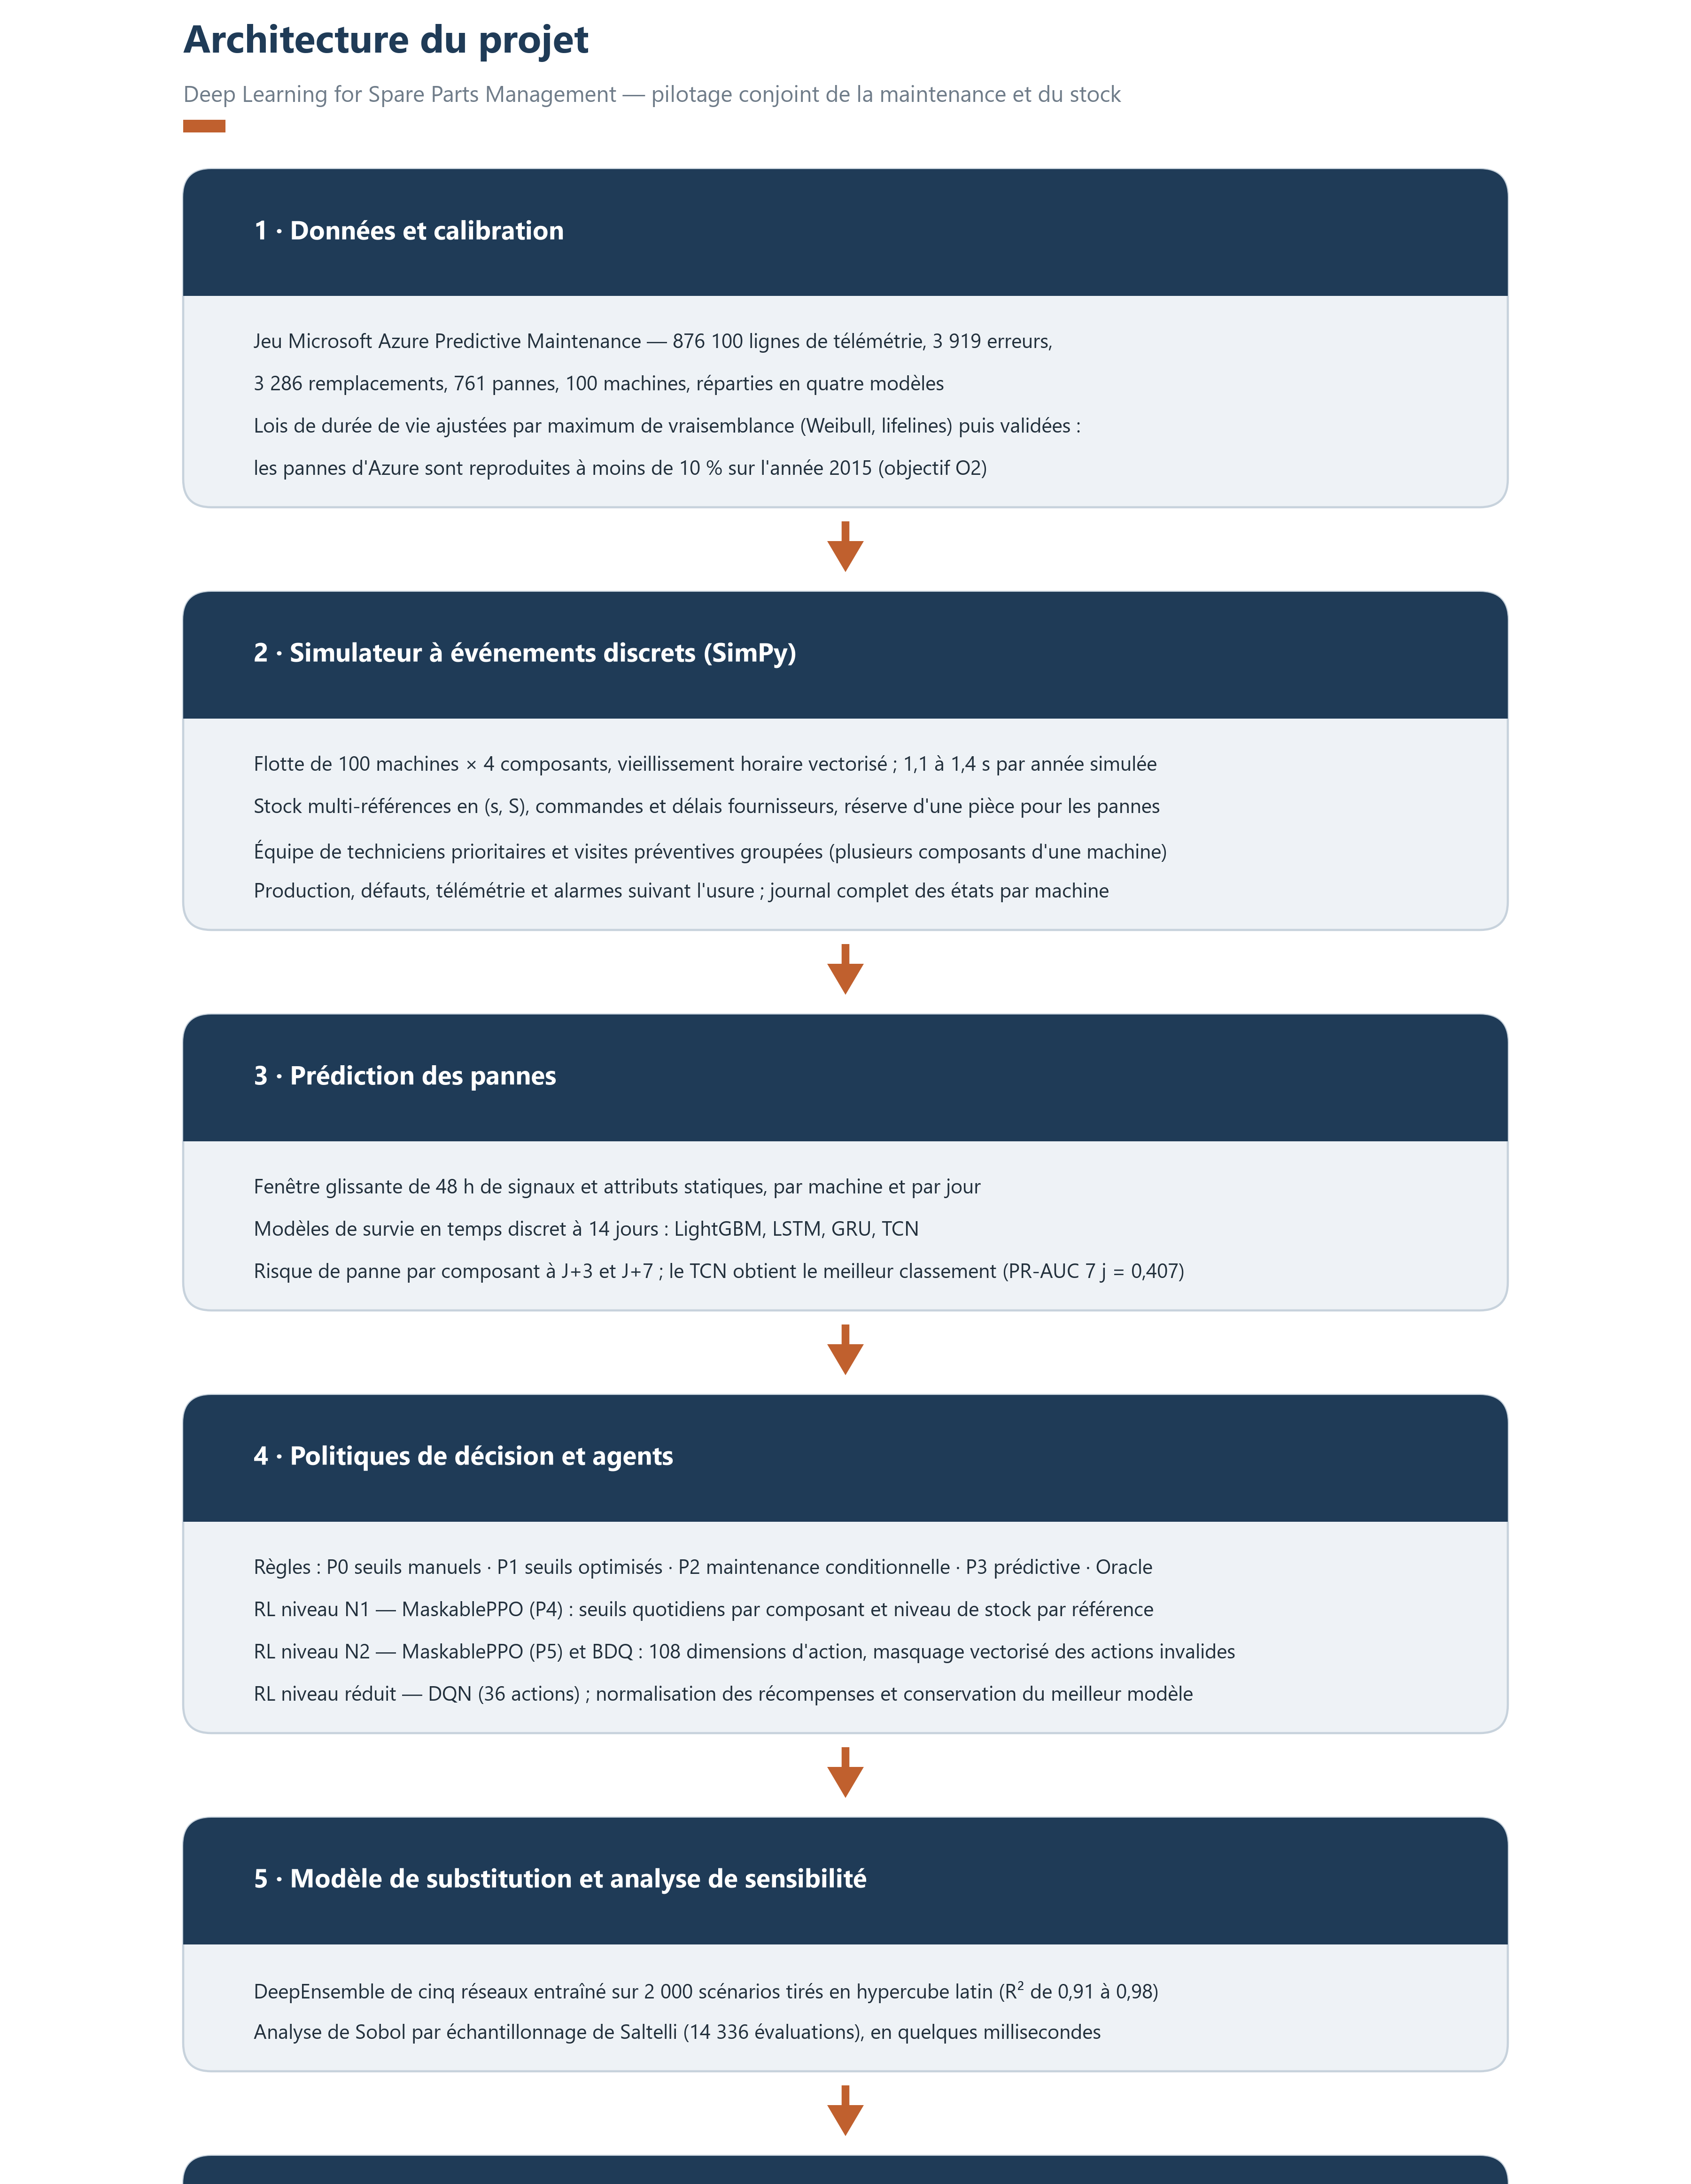
\includegraphics[width=0.78\linewidth]{figures/architecture.png}
\caption{Architecture du projet : données et calibration, simulateur, prédiction, politiques et agents, modèle de substitution, évaluation et restitution.}
\label{fig:architecture}
\end{figure}

% ================================================================ Chapitre 1
\chapter{Données, calibration et simulateur}\label{sec:donnees}

\section{Le jeu de données Azure}

Le jeu Microsoft Azure Predictive Maintenance \cite{azure} confirme les volumes annoncés dans le cahier des charges.

\begin{tabularx}{\linewidth}{@{}L R@{}}
\caption{Volumes du jeu de données Azure}\\
\toprule
\hd{Fichier} & \hd{Lignes} \\
\midrule
Télémétrie horaire (tension, rotation, pression, vibration) & 876\,100 \\
Erreurs non bloquantes & 3\,919 \\
Remplacements de composants & 3\,286 \\
Pannes & 761 \\
Machines & 100 \\
\bottomrule
\end{tabularx}

Les pannes se répartissent entre 192 pour comp1, 259 pour comp2, 131 pour comp3 et 179 pour comp4. Les machines appartiennent à quatre modèles (16, 17, 35 et 32 machines) et ont de 0 à 20 ans. Les moyennes et écarts-types des signaux (170,8 et 15,5 pour la tension, 446,6 et 52,7 pour la rotation, 100,9 et 11,0 pour la pression, 40,4 et 5,4 pour la vibration) correspondent aux niveaux utilisés par le générateur de télémétrie du simulateur.

L'analyse du journal de maintenance révèle une pratique particulière : tous les remplacements sont datés de 6 heures, et les remplacements planifiés ont lieu lors de tournées tous les 15 jours. L'intervalle médian entre deux remplacements planifiés d'un même composant est de 24 à 30 jours, avec un écart-type voisin de la moyenne (environ 50 jours).

\section{Dictionnaire des données}\label{sec:dictionnaire}

Le livrable O1 du cahier des charges demande un jeu de données enrichi accompagné de son dictionnaire. Le jeu enrichi réunit neuf tables, décrites au tableau~\ref{tab:tables-donnees} ; leurs colonnes, leurs types, leurs unités et leur origine sont détaillés dans l'annexe~\ref{sec:dictionnaire-annexe}, dont le tableau~\ref{tab:dictionnaire} constitue le livrable au sens strict.

\begin{tabularx}{\linewidth}{@{}P{2.8cm} P{2.6cm} L P{2.9cm}@{}}
\caption{Tables du jeu de données enrichi}\label{tab:tables-donnees}\\
\toprule
\hd{Table} & \hd{Grain} & \hd{Contenu principal} & \hd{Origine} \\
\midrule
machines & Une ligne par machine & Modèle, âge, famille, postes, cadence, taux de défaut de base, échéance de révision & Azure et ajouts \\
components & Modèle et composant & Régime, intervalle de maintenance, paramètres de Weibull, signal précurseur, lois de durée, type de défaut & Calibration et hypothèses \\
parts & Une ligne par référence & Classe, prix, lois de délai, paramètres de stock & Hypothèses \\
technicians & Équipe & Effectif, calendrier, coût horaire & Hypothèses \\
production & Machine et heure & Pièces produites, défectueuses, rebutées, retouchées & Simulateur, Azure enrichi \\
quality\_events & Un défaut détecté & Type, quantité, composant suspecté, décision & Simulateur \\
events & Un événement & Horodatage, machine, type d'événement, durée, coût & Simulateur \\
state\_intervals & Un séjour dans un état & Machine, état, début, fin, cause & Simulateur \\
ml\_features & Machine et heure & Variables d'apprentissage et étiquettes & Azure et simulateur \\
\bottomrule
\end{tabularx}

La table \texttt{ml\_features} regroupe les variables suivantes :
\begin{itemize}
\item statistiques glissantes des quatre signaux, moyenne et écart-type sur 3 h et 24 h ;
\item nombre d'erreurs par type sur 24 h, taux de défauts sur 8 h et 24 h ;
\item pour chaque composant, temps écoulé depuis le dernier remplacement en heures calendaires, en heures de marche et en millions de tours, ce dernier compteur étant obtenu en cumulant le signal de rotation pendant les heures de marche ;
\item distance à la prochaine échéance de maintenance de chaque composant ;
\item attributs de la machine : âge, modèle, famille, taux d'utilisation ;
\item contexte logistique : stock disponible, commandes en cours et dates d'arrivée prévues ;
\item étiquettes : panne du composant dans les 24 h, 48 h et 7 jours, et temps jusqu'à la panne avec indicateur de censure.
\end{itemize}

Un test automatique vérifie l'absence de fuite d'information temporelle dans ce schéma : aucun attribut n'utilise une donnée postérieure à l'instant de prédiction.

\section{Lois de durée de vie}

Une durée de vie s'étend entre deux remplacements d'un même composant. Elle est complète lorsque le remplacement qui la termine fait suite à une panne, censurée à droite lorsqu'il s'agit d'un remplacement planifié ou de la fin de l'historique. Les lois de Weibull sont ajustées par maximum de vraisemblance avec la bibliothèque lifelines.

\begin{tabularx}{\linewidth}{@{}L R R R R@{}}
\caption{Lois de Weibull ajustées sur Azure}\label{tab:weibull}\\
\toprule
\hd{Composant} & \hd{Forme $\beta$} & \hd{Échelle $\eta$} & \hd{Pannes} & \hd{Durées} \\
\midrule
comp1 & 1,80 & 4\,234 h & 183 & 802 \\
comp2 & 1,50 & 3\,669 h & 256 & 861 \\
comp3 & 1,90 & 5\,093 h & 128 & 806 \\
comp4 & 1,95 & 4\,332 h & 176 & 810 \\
\bottomrule
\end{tabularx}

Les quatre composants ont un paramètre de forme supérieur à 1 : leur taux de panne croît avec l'âge, et la maintenance préventive a donc un intérêt, ce que le cahier des charges demandait de vérifier (§\,3.2). Un modèle de Weibull à temps de vie accéléré précise l'effet des machines : chaque année d'âge réduit la durée de vie des composants d'environ 2~\%, et les modèles 2, 3 et 4 vivent respectivement 17, 46 et 48~\% plus longtemps que le modèle 1.

\begin{figure}[H]
\centering
\begin{tikzpicture}
\begin{axis}[rapport, width=0.86\linewidth, height=6.6cm,
  xlabel={Âge du composant (heures)}, ylabel={Fiabilité $R(t)$},
  xmin=0, xmax=12000, ymin=0, ymax=1.02,
  xtick={0,3000,6000,9000,12000},
  xticklabel style={/pgf/number format/use comma, /pgf/number format/fixed, /pgf/number format/precision=0},
  yticklabel style={/pgf/number format/use comma, /pgf/number format/fixed, /pgf/number format/precision=1},
  legend style={at={(1,1)}, anchor=north east, fill=white, fill opacity=0.9, text opacity=1, legend cell align=left}]
\addplot[primaire, thick, mark=none] table[x=heures, y=comp1, col sep=comma] {data/weibull.csv};
\addplot[accent, thick, mark=none] table[x=heures, y=comp2, col sep=comma] {data/weibull.csv};
\addplot[gris, thick, mark=none] table[x=heures, y=comp3, col sep=comma] {data/weibull.csv};
\addplot[primaire!45, thick, densely dashed, mark=none] table[x=heures, y=comp4, col sep=comma] {data/weibull.csv};
\legend{comp1 ($\beta=1{,}80$), comp2 ($\beta=1{,}50$), comp3 ($\beta=1{,}90$), comp4 ($\beta=1{,}95$)}
\end{axis}
\end{tikzpicture}
\caption{Fiabilité $R(t)=\exp[-(t/\eta)^{\beta}]$ des quatre composants, avec les lois corrigées qui alimentent le simulateur (échelles ramenées à 0,72 -- 0,81 fois les valeurs ajustées). La courbe de comp2 passe sous 0,5 avant 3\,000 heures : c'est le composant qui tombe en panne le plus tôt, ce que la politique P0 doit anticiper.}
\label{fig:weibull}
\end{figure}

\section{Le simulateur}\label{sec:simulateur}

Le simulateur suit l'architecture décrite au §\,5.1 du cahier des charges. Développé avec SimPy, il gère les pannes, interventions et livraisons comme des processus concurrents qui se partagent le stock et l'équipe de techniciens. Le vieillissement des 400 composants est suivi heure par heure de façon vectorisée. La production, les défauts, la télémétrie et les alarmes dépendent de l'usure, qui varie de moins de 1~\% par jour : leurs espérances sont évaluées par blocs de six heures, et juste avant chaque remplacement, puis les quantités sont tirées une fois par jour. Cette organisation conserve la loi des quantités journalières tout en ramenant la simulation d'une année à 1,1 à 1,4 seconde, sous l'exigence de 2 secondes du cahier des charges.

Le simulateur enregistre pour chaque machine l'état hors service dominant de chaque journée et les heures d'arrêt pendant les heures d'ouverture, ce qui alimente les fiches machines de l'application. Il accepte des visites préventives groupées, au cours desquelles un technicien remplace plusieurs composants d'une même machine, comme le fait Azure. Une fenêtre glissante de 48 heures de télémétrie peut être activée pour les politiques prédictives ; elle est normalisée exactement comme les jeux d'apprentissage.

Deux scénarios sont fournis : S1, la flotte hétérogène à deux familles demandée par l'encadrement, et S0, une flotte de machines identiques servant à la validation. Les paramètres de départ sont ceux du chapitre~4 du cahier des charges.

\intertitre{La cible de ruptures du cahier des charges}
Le cahier des charges ajuste les coûts afin que la meilleure politique à seuils fixes connaisse encore 2 à 10~\% de ruptures, sans quoi conserver un stock abondant serait toujours la meilleure décision. Cette cible décrit un régime de tension, non un intervalle à respecter politique par politique, et deux effets la déplacent. D'une part, la fréquence de ruptures se rapporte aux demandes de pièces, qui deviennent rares dès que les pannes chutent : sous la politique P2, les 7,5~ruptures annuelles rapportées à 30 demandes donnent 23,9~\%, très au-dessus de la borne haute, alors que le stock reste plus léger que celui de P1. D'autre part, la politique à seuils fixes réglée à la main (P0) connaît environ 12~\% de ruptures et la politique optimisée (P1) environ 1~\%, de sorte que la famille des politiques à seuils encadre la bande demandée ; c'est cette famille que la consigne visait. La cible est donc respectée à sa racine, et le critère pertinent pour comparer les politiques reste le coût à disponibilité au moins égale, évalué au chapitre~\ref{sec:evaluation}.

\section{Validation du simulateur}\label{sec:validation}

Pour valider le simulateur (objectif O2), nous rejouons la politique observée dans Azure : chaque remplacement planifié du journal est appliqué à sa date, machine par machine, du 1\textsuperscript{er} juin 2014 au 1\textsuperscript{er} janvier 2016, sur 100 machines fonctionnant 24 heures sur 24. Les pannes ne proviennent alors que des lois de Weibull.

Avec les lois ajustées directement, le simulateur produit environ 30~\% de pannes de moins qu'Azure, de façon homogène sur les quatre composants. L'hypothèse de censure indépendante est donc en défaut : les remplacements planifiés d'Azure visent probablement des composants déjà usés, ce qui rend la censure informative et fait surestimer les durées de vie. Nous corrigeons l'échelle de chaque loi par simulation, sur le premier semestre 2015 seulement : le nombre de pannes variant à peu près comme $\eta^{-\beta}$, l'échelle est multipliée à chaque itération par le rapport des pannes simulées et observées, élevé à la puissance $1/\beta$. Les échelles corrigées valent 0,72 à 0,81 fois les échelles ajustées.

\needspace{10\baselineskip}
\begin{tabularx}{\linewidth}{@{}L R R R@{}}
\caption{Écart entre pannes simulées et observées, moyenne sur 8 graines}\label{tab:validation}\\
\toprule
\hd{Composant} & \hd{Lois ajustées, 2\textsuperscript{e} semestre} & \hd{Lois corrigées, 2\textsuperscript{e} semestre} & \hd{Lois corrigées, année} \\
\midrule
comp1 & $-$25,0~\% & $+$18,2~\% & $+$7,9~\% \\
comp2 & $-$30,6~\% & $-$14,3~\% & $-$4,3~\% \\
comp3 & $-$33,7~\% & $-$2,0~\% & $-$3,7~\% \\
comp4 & $-$29,6~\% & $+$6,4~\% & $+$6,4~\% \\
\bottomrule
\end{tabularx}

Sur l'année 2015, l'écart reste inférieur à 10~\% pour chaque composant, ce qui satisfait le critère O2 ; ce résultat inclut toutefois le semestre de calibration. Sur le seul second semestre, que la correction n'a pas vu, deux composants s'écartent de 14 et 18~\%. Cet écart est du même ordre que la variabilité d'Azure elle-même : les pannes réelles de comp1 baissent de 22~\% d'un semestre à l'autre, et l'incertitude de Poisson sur 84 pannes atteint déjà 11~\%. Un critère de 10~\% par semestre est donc proche du bruit statistique des données.

% ================================================================ Chapitre 2
\chapter{Prédiction des pannes}\label{sec:prediction}

\section{Jeux d'apprentissage}

Chaque exemple décrit une machine au début d'une journée : une fenêtre de 48 heures des signaux, des attributs statiques et, pour chaque composant, une cible de survie en temps discret sur 14 jours, censurée par un remplacement préventif ou la fin de l'historique \cite{gensheimer}.

\begin{itemize}
\item \textbf{Données simulées} : cinq années de la flotte S1 sous la politique P0, soit 181\,000 exemples ; trois années servent à l'apprentissage, une à la validation et une au test. Seules 0,13~\% des machines-jours connaissent une panne dans les 24 heures.
\item \textbf{Données réelles} : 36\,300 exemples tirés d'Azure, avec le nombre d'erreurs à la place de l'indicateur de marche et le temps écoulé depuis le dernier remplacement de chaque composant. Le découpage est temporel, comme le prévoit le protocole : janvier à août pour l'apprentissage, septembre et octobre pour la validation, novembre et décembre pour le test.
\end{itemize}

La moyenne et l'écart-type utilisés pour normaliser les quatre signaux Azure sont calculés
uniquement sur la période d'apprentissage (janvier à août), puis appliqués sans réajustement aux
périodes de validation et de test. Cette règle évite que la distribution des périodes évaluées
influence le prétraitement. Les métriques chiffrées ci-dessous proviennent toutefois des artefacts
de la campagne antérieure à cette correction. Les CSV bruts d'Azure n'étant pas présents dans le
dépôt, les modèles n'ont pas pu être réentraînés lors de cette révision ; ces tableaux devront être
régénérés avec le prétraitement corrigé avant le gel d'une version définitive du rapport.

Un remplacement daté de l'instant de prédiction trahit une panne enregistrée au même instant : le temps écoulé depuis le dernier remplacement ne compte donc que les remplacements strictement antérieurs. Un test automatique vérifie l'absence de cette fuite.

\section{Résultats}

Les seuils de décision sont choisis sur la période de validation, les métriques sont mesurées sur le test. L'aire sous la courbe précision-rappel (PR-AUC) se compare à la proportion de pannes : 0,13~\% à 24 heures sur données simulées, 2,1~\% sur Azure.

\begin{tabularx}{\linewidth}{@{}L R R R R@{}}
\caption{Prédiction sur données simulées (année de test)}\label{tab:pred-sim}\\
\toprule
\hd{Modèle} & \hd{F1, 24 h} & \hd{PR-AUC, 24 h} & \hd{F1, 7 jours} & \hd{PR-AUC, 7 jours} \\
\midrule
LightGBM & 0,092 & 0,027 & 0,401 & 0,270 \\
LSTM & 0,150 & 0,101 & 0,439 & 0,365 \\
GRU & 0,165 & 0,098 & 0,444 & 0,405 \\
TCN & 0,146 & 0,099 & 0,455 & 0,407 \\
\bottomrule
\end{tabularx}

\begin{tabularx}{\linewidth}{@{}L R R R R@{}}
\caption{Prédiction sur données réelles Azure (novembre et décembre 2015)}\label{tab:pred-azure}\\
\toprule
\hd{Modèle} & \hd{F1, 24 h} & \hd{PR-AUC, 24 h} & \hd{F1, 7 jours} & \hd{PR-AUC, 7 jours} \\
\midrule
LightGBM & 0,844 & 0,925 & 0,268 & 0,314 \\
LSTM & 0,422 & 0,337 & 0,350 & 0,299 \\
GRU & 0,573 & 0,561 & 0,361 & 0,324 \\
TCN & 0,646 & 0,655 & 0,370 & 0,325 \\
\bottomrule
\end{tabularx}

Sur données simulées, les réseaux de survie dépassent LightGBM aux deux horizons, le TCN et le GRU obtenant le meilleur classement à 7 jours. Sur Azure, LightGBM l'emporte nettement à 24 heures : les pannes de ce jeu synthétique sont précédées d'anomalies franches dans les dernières heures, que des moyennes glissantes sur 3 et 24 heures captent très bien. À 7 jours, horizon qui compte pour la gestion du stock, les réseaux reprennent l'avantage en F1 (0,37 contre 0,27). Le critère O3, qui demandait de dépasser LightGBM, est donc atteint sur données simulées et à 7 jours sur données réelles, mais pas à 24 heures sur données réelles.

\begin{figure}[H]
\centering
\pgfplotsset{pred/.style={rapport, width=\linewidth, height=5.5cm,
  ybar, bar width=6pt, ymin=0, ymax=1.0, enlarge x limits=0.16,
  symbolic x coords={lightgbm,lstm,gru,tcn},
  xtick={lightgbm,lstm,gru,tcn}, xticklabels={LightGBM,LSTM,GRU,TCN},
  yticklabel style={/pgf/number format/use comma, /pgf/number format/fixed, /pgf/number format/precision=1},
  legend style={at={(0.97,0.97)}, anchor=north east, fill=white, fill opacity=0.9, text opacity=1, legend cell align=left, font=\sffamily\footnotesize}}}
\begin{minipage}[t]{0.49\linewidth}
\begin{tikzpicture}
\begin{axis}[pred, title={\sffamily\footnotesize Données simulées (année de test)}, ylabel={PR-AUC}]
\addplot[fill=primaire, draw=none] table[x=modele, y=prauc_24h, col sep=comma] {data/prediction_simulation.csv};
\addplot[fill=accent, draw=none] table[x=modele, y=prauc_7j, col sep=comma] {data/prediction_simulation.csv};
\legend{24 heures, 7 jours}
\end{axis}
\end{tikzpicture}
\end{minipage}\hfill
\begin{minipage}[t]{0.49\linewidth}
\begin{tikzpicture}
\begin{axis}[pred, title={\sffamily\footnotesize Données Azure (novembre, décembre)}, ymax=1.0]
\addplot[fill=primaire, draw=none] table[x=modele, y=prauc_24h, col sep=comma] {data/prediction_azure.csv};
\addplot[fill=accent, draw=none] table[x=modele, y=prauc_7j, col sep=comma] {data/prediction_azure.csv};
\end{axis}
\end{tikzpicture}
\end{minipage}
\caption{Aire sous la courbe précision-rappel de chaque modèle, à 24 heures et à 7 jours. Le TCN signe le meilleur classement à 7 jours sur données simulées (0,407) ; sur Azure, LightGBM reste devant à 24 heures grâce aux anomalies franches qui précèdent les pannes du jeu de données.}
\label{fig:prediction}
\end{figure}

Le premier entraînement de LightGBM donnait un résultat dégénéré, voisin du hasard : avec moins de 200 pannes par composant et un poids des pannes proche de 1\,000, le modèle apprenait les exemples par cœur. Des arbres moins profonds, un poids plafonné et un sous-échantillonnage ont rétabli une référence équitable ; la graine et le mode déterministe sont fixés, si bien que deux exécutions du script produisent exactement les mêmes métriques.

\section{Calibration des probabilités}\label{sec:calibration}

Bien classer les composants ne suffit pas : une probabilité de panne n'oriente la décision que si elle est fiable. La courbe de fiabilité confronte, dans chaque tranche de probabilité prédite, la valeur annoncée à la fréquence réellement observée ; un modèle calibré la place sur la diagonale. L'erreur de calibration attendue (ECE) et le score de Brier, qui mêle fiabilité et pouvoir discriminant, la résument par un nombre.

\begin{tabularx}{\linewidth}{@{}L R R R R@{}}
\caption{Fiabilité des probabilités prédites sur l'année de test simulée}\label{tab:calibration}\\
\toprule
\hd{Modèle} & \hd{Brier, 24 h} & \hd{ECE, 24 h} & \hd{Brier, 7 jours} & \hd{ECE, 7 jours} \\
\midrule
LightGBM & 0,0062 & 0,0066 & 0,0131 & 0,0153 \\
LSTM & 0,0018 & 0,0044 & 0,0140 & 0,0232 \\
GRU & 0,0018 & 0,0045 & 0,0131 & 0,0217 \\
TCN & 0,0017 & 0,0042 & 0,0129 & 0,0223 \\
\bottomrule
\end{tabularx}

À 24 heures, tous les modèles sont bien calibrés : l'écart moyen entre probabilité annoncée et fréquence observée reste sous 0,7 point. À 7 jours, l'écart s'élargit jusqu'à 2,3 points pour le LSTM. La figure~\ref{fig:calibration} en montre la cause : au-delà de 0,8, les quatre modèles surestiment le risque, la tranche annoncée à 0,95 ne contenant que 40 à 52~\% de pannes réelles. Cette prudence ne coûte guère — mieux vaut déclencher une maintenance de trop que manquer une panne — mais elle justifie que la politique prédictive P3 règle un seuil sur le risque au lieu de lire la probabilité comme une fréquence. Le classement, lui, reste excellent : l'indice de concordance des trois réseaux à 7 jours dépasse 0,94.

\begin{figure}[H]
\centering
\begin{tikzpicture}
\begin{axis}[rapport, width=0.70\linewidth, height=7.2cm,
  xlabel={Probabilité prédite}, ylabel={Fréquence observée},
  xmin=0, xmax=1, ymin=0, ymax=1,
  xticklabel style={/pgf/number format/use comma, /pgf/number format/fixed, /pgf/number format/precision=1},
  yticklabel style={/pgf/number format/use comma, /pgf/number format/fixed, /pgf/number format/precision=1},
  legend style={at={(0.03,0.97)}, anchor=north west, fill=white, fill opacity=0.9, text opacity=1}]
\addplot[gris!60, densely dotted, domain=0:1, samples=2] {x};
\addplot[gris, mark=square*, mark size=1.6pt, thick] table[x=proba, y=observe, col sep=comma] {data/calibration_simulation_lightgbm.csv};
\addplot[primaire, mark=*, mark size=1.8pt, thick] table[x=proba, y=observe, col sep=comma] {data/calibration_simulation_tcn.csv};
\addplot[accent, mark=triangle*, mark size=2.1pt, thick] table[x=proba, y=observe, col sep=comma] {data/calibration_simulation_gru.csv};
\addplot[primaire!45, mark=diamond*, mark size=2.1pt, thick] table[x=proba, y=observe, col sep=comma] {data/calibration_simulation_lstm.csv};
\legend{Diagonale, LightGBM, TCN, GRU, LSTM}
\end{axis}
\end{tikzpicture}
\caption{Courbes de fiabilité à 7 jours sur l'année de test simulée : probabilité prédite contre fréquence observée, par tranches de largeur 0,1. Un modèle parfaitement calibré suivrait la diagonale ; les quatre surestiment le risque au-delà de 0,8.}
\label{fig:calibration}
\end{figure}

% ================================================================ Chapitre 3
\chapter{Politiques et agents décisionnels}\label{sec:agents}

\section{Politiques de référence}\label{sec:references}

\begin{itemize}
\item \textbf{P0}, seuils fixes réglés à la main : stock en $(s,S)$ selon le scénario, maintenance systématique aux intervalles constructeur, une pièce de chaque référence réservée aux pannes.
\item \textbf{P1}, seuils fixes optimisés : recherche aléatoire de 40 combinaisons des seuils $(s,S)$ et des facteurs d'intervalle de maintenance, évaluées sur les mêmes graines. Sur les graines de réglage, le coût annuel passe de 57\,600 à 53\,700 UR et les ruptures de 16 à 1~\%.
\item \textbf{P2}, maintenance conditionnelle : remplacement lorsque le signal associé au composant dérive, lorsque le taux de défauts dépasse un seuil, ou à 1,5 fois l'intervalle.
\item \textbf{P3}, politique prédictive sans apprentissage par renforcement : le réseau de survie qui classe le mieux les pannes à 7 jours estime le risque de chaque composant. Un composant est remplacé lorsque son risque de panne à 3 jours dépasse un seuil ou lorsqu'il atteint un multiple donné de son intervalle de maintenance, et le stock est recomplété jusqu'à la demande prévue sur le délai fournisseur, augmentée d'un stock de sécurité. Sans la seconde règle, P3 laissait vieillir les composants : le taux de défauts passait de 2,4 à 3,1~\% et le rebut coûtait 10\,000 UR de plus par an. Ses trois paramètres sont réglés sur une grille de 18 combinaisons, avec les graines de P1 : la grille retient un seuil de risque de 2~\%, un remplacement d'office à 1,5 fois l'intervalle et une marge de stock réduite à une pièce, pour un coût de 52\,200 UR sur ces graines.
\item \textbf{Oracle} : remplace chaque composant à 70~\% de sa durée de vie réelle et commande les pièces dont il sait qu'elles serviront ; c'est une borne qu'aucune politique réaliste ne peut atteindre.
\end{itemize}

\section{Apprentissage par renforcement}\label{sec:apprentissage}

Les politiques précédentes fixent une règle, que l'on règle ensuite ; les agents décrits ici apprennent cette règle directement. Le chapitre présente la formulation du problème, les niveaux d'action offerts aux agents, les algorithmes retenus et les courbes d'apprentissage.

% Agents décisionnels : apprentissage par renforcement (section « Apprentissage par renforcement », chapitre 3)
\subsection{Formulation de l'apprentissage}\label{sec:rl}

L'agent décide une fois par jour, au début de la journée, à partir de l'état observable de la flotte. Un épisode couvre une année, soit 365 décisions, et chaque épisode tire une nouvelle graine du simulateur : l'agent ne revoit jamais deux fois la même suite de pannes. La récompense d'une journée est l'opposé de son coût total, qui regroupe les huit postes du cahier des charges (stockage, achats, urgences, main-d'œuvre, surcoût correctif, arrêts, rebut et retouche), divisé par 150 pour ramener les récompenses vers l'unité. Maximiser la somme des récompenses revient donc exactement à minimiser le coût annuel, sans pondération arbitraire entre coût et disponibilité : les arrêts sont valorisés par la marge perdue.

L'observation ne contient que des grandeurs connues d'un responsable de maintenance réel : stock, commandes en cours et machines en attente pour chaque référence, avancement de chaque composant par rapport à son intervalle de maintenance (moyenne, maximum et part des composants au-delà de 80 et 100~\%), part des machines en service, en attente de pièce ou de technicien, techniciens libres, taux de défauts et alarmes des dernières 24 heures, avancement de l'année. Deux grandeurs d'atelier complètent cette base : le risque de panne estimé par le réseau de survie pour chaque composant, qui déclenche la maintenance de P3, et la dérive normalisée du signal de chaque composant, qui déclenche la maintenance conditionnelle de P2. Les durées de vie réelles des composants restent cachées. Toutes les grandeurs sont normalisées par des valeurs de référence du scénario, ce qui donne 55 variables, contre 39 sans ces deux blocs.

\subsection{Trois niveaux d'action}

Le cahier des charges prévoyait deux niveaux d'action (§\,5.3). Un troisième, plus simple, a été ajouté pour pouvoir appliquer un DQN classique, qui ne sait traiter qu'un petit nombre d'actions discrètes.

\begin{tabularx}{\linewidth}{@{}P{2.3cm} L P{3.6cm}@{}}
\caption{Niveaux d'action proposés aux agents}\label{tab:niveaux}\\
\toprule
\hd{Niveau} & \hd{Décision quotidienne} & \hd{Taille de l'espace} \\
\midrule
Réduit & Un seuil de maintenance commun à tous les composants et un multiplicateur de stock commun à toutes les références, chacun parmi six valeurs & 36 actions \\
N1 & Un seuil de maintenance par composant (0,6 à 1,5 fois l'intervalle, ou jamais) et un niveau de recomplètement par référence (0,5 à 3 fois le niveau de référence) & $6^8 \approx 1{,}7$ million de combinaisons \\
N2 & Quantité commandée et commande urgente pour chaque référence, et pour chaque machine : ne rien faire ou remplacer l'un de ses quatre composants & plus de $10^{76}$ combinaisons \\
\bottomrule
\end{tabularx}

Au niveau N1, l'agent règle chaque jour les paramètres d'une politique à seuils, que le simulateur applique ensuite. Ce niveau reste lisible pour un responsable de maintenance : il voit à tout moment quels seuils l'agent a retenus. Au niveau N2, l'agent prend lui-même chaque décision. Les actions impossibles ou absurdes y sont masquées : maintenance d'une machine déjà arrêtée, d'un composant dont la pièce manque ou qui n'a pas atteint la moitié de son intervalle, ou alors qu'aucun technicien n'est libre. Pour ce niveau, l'observation est complétée, pour chaque machine, par son état, le risque, la dérive et l'avancement de ses quatre composants, soit 1\,355 variables.

\subsection{Algorithmes}

\intertitre{MaskablePPO pour P4 et P5}
PPO \cite{ppo} est un algorithme acteur-critique robuste aux espaces d'actions discrets multiples. Sa variante MaskablePPO de la bibliothèque sb3-contrib \cite{sb3} exclut les actions invalides de la distribution de l'acteur, ce qui accélère nettement l'apprentissage par rapport à une pénalité \cite{masking}. Les deux agents partagent leurs réglages : huit environnements en parallèle, 365 pas par environnement entre deux mises à jour, lots de 730 transitions, taux d'apprentissage $3\times10^{-4}$, facteur d'actualisation 0,995 (horizon effectif de 200 jours, du même ordre que les délais et les durées de vie). P4 dispose de 300\,000 pas, soit environ 820 années simulées, et d'un coefficient d'entropie de 0,01 ; P5 de 300\,000 pas également, mais sans bonus d'entropie. Chaque agent est en outre entraîné sur trois graines, et l'horizon de ses épisodes croît de 90 jours à une année complète au fil de l'apprentissage ; la politique retenue est celle dont le coût annuel moyen sur cinq graines de validation est le plus faible. Ces choix, ainsi que la normalisation des récompenses et la conservation du meilleur modèle, sont justifiés plus bas. Au niveau N2, la loi masquée de sb3-contrib traite les 108 dimensions de l'action une à une et coûtait 77~ms par décision, quinze fois le temps de simulation d'une journée ; une version vectorisée, dont un test vérifie qu'elle donne les mêmes probabilités, ramène ce temps à 1,5~ms.

\intertitre{DQN au niveau réduit}
Le DQN \cite{dqn} de Stable-Baselines3 sert de référence : réseau de deux couches de 64 neurones, mémoire de 200\,000 transitions, exploration $\varepsilon$ décroissante sur les 10 premiers pourcents de l'apprentissage, 300\,000 pas.

\intertitre{Branching Dueling Q-Network}
Un DQN classique estime une valeur par action ; au niveau N2, il devrait en estimer plus de $10^{76}$. L'architecture à branches de Tavakoli et al. \cite{bdq} contourne cette explosion : un tronc commun de deux couches de 256 neurones alimente une valeur d'état et, pour chaque dimension de l'action, une tête d'avantages. Le nombre de sorties croît alors avec la somme des tailles des dimensions (près de 600) et non avec leur produit. La cible d'apprentissage suit le double DQN, en moyenne sur les branches, et les actions invalides sont masquées dans chaque branche. Ce réseau, absent des bibliothèques courantes, a été écrit directement avec PyTorch ; les sorties de toutes les branches sont rangées dans un même tableau pour éviter une boucle sur la centaine de branches. L'apprentissage dure 200\,000 pas, avec une mise à jour tous les quatre pas sur des lots de 64 transitions, une mémoire de 100\,000 transitions, un taux d'apprentissage de $10^{-4}$ et une exploration $\varepsilon$ qui décroît de 1 à 0,05 sur les 30 premiers pourcents.

\intertitre{Point de départ des agents N2}
Un agent non entraîné choisit presque uniformément entre les options de chaque dimension : au niveau N2, il commande chaque jour des quantités aléatoires et envoie en maintenance quatre machines sur cinq. Ces premières années coûtent plus de 600\,000 UR, dix fois le coût normal, et la multitude d'interventions ralentit la simulation au point de ramener l'apprentissage à une vingtaine de pas par seconde. Nous ajoutons donc, avant apprentissage, un biais aux sorties des deux agents N2 qui rend l'option « ne rien faire » largement majoritaire ; l'exploration du BDQ tire ses actions aléatoires selon ce même biais. L'agent part ainsi d'une politique prudente et apprend quand s'en écarter, ce qui ne restreint aucune décision. Le bonus d'entropie habituel a en revanche été écarté au niveau N2 : sommé sur 108 dimensions, il pousse l'acteur vers des choix uniformes, c'est-à-dire précisément vers les années absurdes que le biais initial écarte.

\intertitre{Normalisation des récompenses}
Sans normalisation, les deux agents piétinaient. Le premier apprentissage de P4, mené sans précaution particulière, en donne la mesure : le coût moyen des épisodes est passé de 53\,800 à 53\,400 UR en 300\,000 pas, autant dire qu'il n'a pas bougé. Dans les deux cas, la variance des retours expliquée par le critique restait nulle, si bien que les avantages estimés n'étaient guère que du bruit. Les retours, de l'ordre de $-200$, varient beaucoup d'une année à l'autre ; les récompenses sont donc divisées par l'écart-type courant des retours, ce qui ramène les cibles du critique vers l'unité. La variance expliquée est alors passée à plus de 0,5 dès les premières mises à jour. Les deux agents ont été réentraînés ainsi, et le modèle conservé est celui dont le coût annuel moyen des derniers épisodes est le plus faible, et non le dernier. Chaque épisode est d'abord ramené à une année, en divisant sa récompense par sa durée, sinon le curriculum retiendrait le tout premier tirage : ses épisodes de quatre-vingt-dix jours, plus courts, paraissent artificiellement moins coûteux que des années entières.

\subsection{Courbes d'apprentissage}

La figure~\ref{fig:apprentissage} suit le coût annuel moyen des derniers épisodes au fil de l'apprentissage. Ces épisodes sont joués avec la politique stochastique de l'agent, ou avec son exploration pour les deux DQN, et sur des graines chaque fois nouvelles : la courbe mesure la progression, pas la performance finale, que le chapitre~\ref{sec:evaluation} évalue sur des années communes à toutes les politiques.

\begin{figure}[H]
\centering
\pgfplotsset{courbe/.style={rapport, width=\linewidth, height=6cm,
  xlabel={Pas d'apprentissage (milliers)},
  x filter/.expression={x/1000}, y filter/.expression={y/1000}, xmin=0,
  xticklabel style={/pgf/number format/use comma, /pgf/number format/fixed, /pgf/number format/precision=0},
  yticklabel style={/pgf/number format/use comma, /pgf/number format/fixed, /pgf/number format/precision=0},
  legend style={at={(1,1)}, anchor=north east, fill=white, fill opacity=0.9, text opacity=1},
  legend cell align=left}}
\begin{minipage}[t]{0.49\linewidth}
\begin{tikzpicture}
\begin{axis}[courbe, xmax=300, ymin=50, ymax=64, ylabel={Coût annuel moyen (milliers d'UR)},
  title={\sffamily\footnotesize Niveaux réduit et N1}]
\addplot[primaire, thick, mark=none] table[x=pas, y=cout_annuel, col sep=comma] {data/courbe_maskable_ppo_n1_s1_nominal_s0.csv};
\addplot[primaire!45, mark=none, densely dashed] table[x=pas, y=cout_annuel, col sep=comma] {data/courbe_maskable_ppo_n1_sans_normalisation.csv};
\addplot[gris, mark=none] table[x=pas, y=cout_annuel, col sep=comma] {data/courbe_dqn_reduced_s1_nominal_s0.csv};
\addplot[gris!70, mark=none, densely dotted, domain=0:300000] {52136};
\legend{P4, P4 sans normalisation, DQN, P1 (évaluation)}
\end{axis}
\end{tikzpicture}
\end{minipage}\hfill
\begin{minipage}[t]{0.49\linewidth}
\begin{tikzpicture}
\begin{axis}[courbe, xmax=300, ymin=40, ymax=280,
  title={\sffamily\footnotesize Niveau N2}]
\addplot[accent, thick, mark=none] table[x=pas, y=cout_annuel, col sep=comma] {data/courbe_maskable_ppo_n2_s1_nominal_s0.csv};
\addplot[accent!60, mark=none, densely dashed] table[x=pas, y=cout_moy, col sep=comma] {data/courbe_bdq.csv};
\addplot[gris!70, mark=none, densely dotted, domain=0:300000] {52136};
\legend{P5, BDQ, P1 (évaluation)}
\end{axis}
\end{tikzpicture}
\end{minipage}
\caption{Coût annuel moyen des épisodes d'apprentissage : moyenne glissante des 100 derniers épisodes pour PPO et DQN, des 20 derniers pour le BDQ. Le pointillé rappelle le coût de P1 mesuré lors de l'évaluation finale.}
\label{fig:apprentissage}
\end{figure}

Une fois les récompenses normalisées, P5 progresse nettement : sa courbe part de 109\,200 UR et descend jusqu'à environ 66\,700 UR en fin d'apprentissage ; la durée d'apprentissage n'est donc plus ce qui le limite. P4, dont l'espace d'action est bien plus étroit, part de 62\,300 UR, culmine à 63\,500 UR vers 26\,000 pas, puis redescend et se stabilise un peu au-dessus de 53\,200 UR, sans que la normalisation change grand-chose à son niveau final (53\,400 UR sans elle) : les seuils quotidiens qu'il règle, de la même famille que ceux de P1, ne lui laissent que peu de marge. Le BDQ, lui, décroche franchement : sa courbe moyenne culmine à environ 243\,000 UR vers 103\,000 pas, avant de refluer régulièrement à mesure que l'exploration s'éteint pour terminer autour de 97\,000 UR : les valeurs de ses 108 branches sont apprises sur une récompense commune à toute la flotte, et l'effet d'une décision isolée, comme l'entretien d'une machine, se perd dans le bruit des pannes des 99 autres. Le DQN, enfin, oscille sans tendance entre 55\,100 et 61\,300 UR et termine à 56\,200 UR : un seuil commun à tous les composants et un niveau de stock commun à toutes les références ne laissent guère de marge.

La figure~\ref{fig:apprentissage} suit une seule graine par agent ; entraîner trois fois le même agent donne trois courbes différentes. La figure~\ref{fig:dispersion} rassemble pour chaque agent la moyenne des trois graines et l'étendue qui les sépare.

\begin{figure}[H]
\centering
\pgfplotsset{disp/.style={rapport, width=\linewidth, height=5.0cm,
  x filter/.expression={x/1000}, y filter/.expression={y/1000}, xmin=0, xmax=305,
  xticklabel style={/pgf/number format/use comma, /pgf/number format/fixed, /pgf/number format/precision=0},
  yticklabel style={/pgf/number format/use comma, /pgf/number format/fixed, /pgf/number format/precision=0},
  legend style={at={(0.02,0.03)}, anchor=south west, fill=white, fill opacity=0.85,
    text opacity=1, draw=none, font=\sffamily\scriptsize, legend cell align=left}}}
\begin{minipage}[t]{0.49\linewidth}
\begin{tikzpicture}
\begin{axis}[disp, ymin=52, ymax=65, ylabel={Coût annuel moyen (milliers d'UR)},
  title={\sffamily\footnotesize P4, niveau N1}]
\addplot[name path=p4hi, draw=none, forget plot] table[x=pas, y=cout_max, col sep=comma] {data/courbe_p4.csv};
\addplot[name path=p4lo, draw=none, forget plot] table[x=pas, y=cout_min, col sep=comma] {data/courbe_p4.csv};
\addplot[primaire!20] fill between[of=p4hi and p4lo];
\addplot[primaire, thick, mark=none] table[x=pas, y=cout_moy, col sep=comma] {data/courbe_p4.csv};
\legend{Étendue sur trois graines, Moyenne}
\end{axis}
\end{tikzpicture}
\end{minipage}\hfill
\begin{minipage}[t]{0.49\linewidth}
\begin{tikzpicture}
\begin{axis}[disp, ymin=62, ymax=115, title={\sffamily\footnotesize P5, niveau N2}]
\addplot[name path=p5hi, draw=none, forget plot] table[x=pas, y=cout_max, col sep=comma] {data/courbe_p5.csv};
\addplot[name path=p5lo, draw=none, forget plot] table[x=pas, y=cout_min, col sep=comma] {data/courbe_p5.csv};
\addplot[accent!20] fill between[of=p5hi and p5lo];
\addplot[accent, thick, mark=none] table[x=pas, y=cout_moy, col sep=comma] {data/courbe_p5.csv};
\end{axis}
\end{tikzpicture}
\end{minipage}

\vspace{0.7em}

\begin{minipage}[t]{0.49\linewidth}
\begin{tikzpicture}
\begin{axis}[disp, ymin=54, ymax=64, xlabel={Pas d'apprentissage (milliers)},
  ylabel={Coût annuel moyen (milliers d'UR)}, title={\sffamily\footnotesize DQN, niveau réduit}]
\addplot[name path=dqnhi, draw=none, forget plot] table[x=pas, y=cout_max, col sep=comma] {data/courbe_dqn.csv};
\addplot[name path=dqnlo, draw=none, forget plot] table[x=pas, y=cout_min, col sep=comma] {data/courbe_dqn.csv};
\addplot[gris!30] fill between[of=dqnhi and dqnlo];
\addplot[gris, thick, mark=none] table[x=pas, y=cout_moy, col sep=comma] {data/courbe_dqn.csv};
\end{axis}
\end{tikzpicture}
\end{minipage}\hfill
\begin{minipage}[t]{0.49\linewidth}
\begin{tikzpicture}
\begin{axis}[disp, ymin=60, ymax=280, xlabel={Pas d'apprentissage (milliers)},
  title={\sffamily\footnotesize BDQ, niveau N2}]
\addplot[name path=bdqhi, draw=none, forget plot] table[x=pas, y=cout_max, col sep=comma] {data/courbe_bdq.csv};
\addplot[name path=bdqlo, draw=none, forget plot] table[x=pas, y=cout_min, col sep=comma] {data/courbe_bdq.csv};
\addplot[accent!18] fill between[of=bdqhi and bdqlo];
\addplot[accent!60, thick, mark=none] table[x=pas, y=cout_moy, col sep=comma] {data/courbe_bdq.csv};
\end{axis}
\end{tikzpicture}
\end{minipage}
\caption{Coût annuel moyen sur les trois graines d'entraînement de chaque agent, et étendue entre la meilleure et la pire graine au même pas. Une enveloppe étroite signale un apprentissage reproductible : en fin d'apprentissage, l'écart entre graines vaut environ 150 UR pour le DQN, 1\,000 UR pour P4, de l'ordre du millier pour P5, et 2\,200 UR pour le BDQ — un écart qui dépasse 100\,000 UR au plus fort de sa phase instable.}
\label{fig:dispersion}
\end{figure}

Les écarts de reproductibilité suivent la taille de l'espace d'action. En fin d'apprentissage, l'étendue entre les trois graines vaut environ 150 UR pour le DQN, dont l'action tient en 36 choix, et 1\,000 UR pour P4, dont l'espace dépasse pourtant le million de combinaisons : ces deux agents convergent vers des courbes presque superposées. P5, à plus de $10^{76}$ actions effectives, garde une enveloppe de l'ordre du millier d'UR. Le BDQ se détache nettement, avec 2\,200 UR entre ses graines en fin d'apprentissage, et plus de 100\,000 UR lorsque sa courbe est au plus haut : l'initialisation des poids d'un réseau à branches et l'ordre des transitions rencontrées pèsent plus lourd que pour un acteur-critique. Ce classement ne change pas la comparaison du chapitre~\ref{sec:evaluation}, où le BDQ reste loin derrière P1 quelle que soit la graine, mais il invite à lire sa courbe moyenne avec prudence.

\intertitre{Jouer l'action la plus probable ou tirer les actions}
Une politique PPO est une loi de probabilité sur les actions. L'usage veut qu'on l'évalue en jouant son mode, l'action la plus probable de chaque dimension, mais ce mode peut s'écarter beaucoup de la politique apprise. Au niveau N2, « ne rien commander » reste l'option la plus probable de chaque référence : l'agent apprend à commander certains jours seulement, et son mode ne commande jamais. Joué ainsi, P5 coûte 401\,900 UR par an sur les graines de réglage, contre 65\,000 UR en tirant ses actions. Pour chaque agent PPO, le mode de jeu est donc choisi sur les graines de réglage de P1 et P3, jamais sur celles de l'évaluation finale, et le tirage est initialisé par la graine de la simulation pour rester reproductible. Le tirage l'emporte nettement pour P5 (65\,000 UR contre 401\,900 UR pour le mode) ; pour P4, où l'écart est plus ténu, c'est en revanche le mode qui l'emporte (54\,800 UR contre 55\,600 UR) : au niveau N1, l'action la plus probable de chaque dimension reste un seuil de maintenance sensé, alors qu'au niveau N2 le mode « ne rien faire » est inutilisable.


% ================================================================ Chapitre 4
\chapter{Évaluation, substitution et robustesse}\label{sec:evaluation}

\section{Évaluation comparative des politiques}\label{sec:evaluation-comparative}

% Évaluation : protocole, scénario nominal et robustesse (sous-sections de « Évaluation comparative », chapitre 4)
\subsection{Protocole}

Le protocole est celui du §\,7.3 du cahier des charges. Chaque politique est simulée sur les mêmes 30 années, de graines 9000 à 9029, qu'aucun réglage ni apprentissage n'a utilisées. Les nombres aléatoires communs font que deux politiques affrontent exactement les mêmes durées de vie et les mêmes aléas de délai : l'écart observé sur une graine ne doit rien au hasard du tirage. Les moyennes sont accompagnées de leur intervalle de confiance à 95~\%, et l'écart de coût de chaque politique à P1 est testé par un test de Wilcoxon apparié sur les 30 années.

\needspace{18\baselineskip}
\subsection{Scénario nominal}

\begin{tabularx}{\linewidth}{@{}l R P{3.1cm} r r r r r@{}}
\caption{Indicateurs moyens sur 30 années, scénario S1 nominal}\label{tab:evaluation}\\
\toprule
\hd{Pol.} & \hd{Coût (UR)} & \hd{IC 95~\%} & \hd{TRS} & \hd{Dispo.} & \hd{Ruptures} & \hd{Attente (h)} & \hd{$p$} \\
\midrule
\lignes{data/tableau_evaluation.tex}
\bottomrule
\end{tabularx}

La colonne $p$ donne la probabilité, sous l'hypothèse d'une absence d'écart avec P1, d'observer un écart de coût au moins aussi marqué. Les ruptures sont la part des demandes de pièces après panne que le stock n'a pas pu servir immédiatement ; l'attente est la durée moyenne d'attente de pièce par réparation, en heures. Le test de Wilcoxon conclut à une différence significative dès que celle-ci est réelle, mais il ne dit pas dans quel sens ; le test d'équivalence du tableau~\ref{tab:tost}, mené sur la même marge de $\pm 2$~\%, sépare donc les politiques qui s'écartent de P1 vers le mieux de celles qui s'en écartent vers le pire.

\needspace{13\baselineskip}
\begin{tabularx}{\linewidth}{@{}l R r l@{}}
\caption{Test d'équivalence (TOST) du coût annuel contre P1, marge $\pm 2$~\%, scénario S1 nominal}\label{tab:tost}\\
\toprule
\hd{Pol.} & \hd{Écart moyen (UR)} & \hd{Écart (\% de P1)} & \hd{Verdict} \\
\midrule
\lignes{data/tableau_tost.tex}
\bottomrule
\end{tabularx}

\intertitre{La prédiction réduit le coût, la surveillance d'état davantage encore}
P3, qui s'appuie sur le réseau de survie, coûte 49\,200 UR par an, 5,6~\% de moins que P1, et l'écart est significatif ($p < 10^{-6}$). Il ramène les pannes de 189 à 39 par an et porte la disponibilité à 99,25~\%, la meilleure des politiques réalistes. La maintenance conditionnelle P2 fait pourtant mieux, avec 47\,100 UR, soit 9,6~\% de moins que P1, sans aucun réglage. Elle ramène les pannes à 30 par an et, avec si peu de pannes, se contente des niveaux de stock de P0 : la valeur moyenne du stock est de 208 UR pour P2, contre 847 pour P3 et 1\,105 pour P1. Elle surveille aussi le taux de défauts, que le réseau de survie ignore : P3 laisse les composants s'user un peu plus, avec 2,4~\% de pièces défectueuses contre 2,2~\% pour P2. L'avantage de P2 tient donc moins à la qualité de sa détection qu'à ce qu'elle observe : la dérive du signal propre à chaque composant, que le simulateur relie directement à l'usure, est une information plus directe qu'un risque de panne estimé.

\intertitre{La fréquence de ruptures se lit avec le nombre de pannes}
P2 présente 23,9~\% de ruptures, mais sur 30 demandes seulement : cela représente 7,5 ruptures par an, contre 2,1 pour P1. Ces attentes, longues (110 heures en moyenne) mais rares, ne pèsent presque pas sur le TRS, proche de celui de P1 et de P3 (96,7 à 96,8~\%).

\intertitre{Les agents d'apprentissage par renforcement n'atteignent pas P1}
Les deux agents les plus proches de P1 sont ceux dont l'espace d'action se réduit à des seuils. P4, au niveau N1, est le plus proche : il coûte 52\,800 UR par an, seulement 1,3~\% de plus que P1, écart significatif mais d'ampleur marginale ($p = 0{,}019$), pour un TRS légèrement inférieur (96,44 contre 96,69~\%), un stock plus léger que P1 (631 UR contre 1\,105), davantage de ruptures (3,9 contre 1,1~\%) et un peu plus de pannes (203 contre 189 par an). Le DQN du niveau réduit, lui, coûte 54\,900 UR, 5,4~\% de plus que P1 : il fait ainsi à peine mieux que P0 (55\,400 UR), dont il partage le TRS (96,1 contre 96,1~\%), avec un stock à peine plus léger (172 UR contre 187) et un peu moins de pannes (177 contre 181 par an). Leur point commun est un espace d'action paramétrique : le DQN règle chaque jour un seuil d'âge commun à tous les composants et un niveau de stock commun, P4 un seuil d'âge et un niveau de stock par composant, c'est-à-dire une politique de la même famille que P1. Dans les deux cas, la maintenance préventive se déclenche sur l'âge rapporté à l'intervalle, non sur l'état observé du composant — là où P2 et P3 trouvent l'essentiel de leur avantage. Reste donc à savoir si ce vocabulaire interdit d'atteindre P1, ou si les agents l'ont simplement mal exploité.

\intertitre{Ce que le répertoire d'actions de chaque agent laisse atteindre}
Un agent ne peut pas descendre sous le meilleur coût de son propre répertoire. On appelle \emph{plancher de représentation} d'un espace d'action $A$ le coût de sa meilleure politique \emph{constante} — un réglage unique tenu toute l'année — évalué sur les mêmes trente années. L'écart de l'agent à ce plancher mesure ce qu'il n'a pas su tirer d'un répertoire qui le lui permettait ; l'écart du plancher à P1, ce que ce répertoire, sous sa forme la plus simple, laisse au-dessus de la référence. Les deux parts se somment exactement à l'écart observé. Pour l'espace réduit du DQN, les 36 actions sont énumérées, si bien que le plancher y est \emph{exact} ; pour l'espace N1 de P4 ($6^8 = 1\,679\,616$ actions), une montée de coordonnée depuis quatre départs en fournit un majorant réalisable — le coût retenu est celui d'une politique effectivement jouable.

\needspace{14\baselineskip}
\begin{tabularx}{\linewidth}{@{}l L R R R R@{}}
\caption{Décomposition de l'écart de coût de chaque agent à P1, scénario S1 nominal. Le plancher est le meilleur coût atteint par une politique constante de l'espace d'action ; l'écart d'apprentissage est ce que l'agent laisse entre lui et ce plancher, l'écart de représentation ce que le plancher laisse au-dessus de P1. Les pourcentages se rapportent au coût de P1.}\label{tab:plancher}\\
\toprule
\hd{Pol.} & \hd{Espace d'action} & \hd{Coût agent} & \hd{Plancher} & \hd{Écart d'apprentissage} & \hd{Écart de représentation} \\
\midrule
\lignes{data/tableau_plancher.tex}
\bottomrule
\end{tabularx}

Le tableau tranche, et de deux façons opposées. Le meilleur réglage fixe de l'espace réduit coûte 54\,279 UR, soit 4,1~\% au-dessus de P1 : le vocabulaire du DQN — seuil commun aux quatre composants, point de commande \emph{dérivé} du niveau de stock — ne peut pas rejoindre P1, et cette restriction explique 2\,143 UR des 2\,796 UR d'écart du DQN, l'apprentissage n'en portant que 652. La conclusion s'inverse pour l'espace N1 : la montée de coordonnée y trouve un réglage fixe à 50\,185 UR, \emph{1\,952 UR sous P1}. Le répertoire de P4 contient donc une politique qui satisfait le critère O4 : son écart observé de 662 UR se scinde en 2\,614 UR d'apprentissage et $-$1\,952 UR de représentation, la part de représentation étant \emph{négative} puisque son meilleur réglage fixe bat P1. Autrement dit, l'agent laisse inexploité l'avantage de 1\,952 UR que ses seuils lui offraient, et reste encore 2\,614 UR au-dessus du réglage fixe pourtant accessible dans son propre espace. Les politiques constantes formant un sous-ensemble de celles de l'espace, la part d'apprentissage est un \emph{minorant} et celle de représentation un \emph{majorant} : ces deux bornes vont dans le sens des conclusions ci-dessus.

Le verdict du critère O4 reste donc négatif, mais de justesse pour P4, comme le rappelle la conclusion. Son diagnostic, en revanche, n'est plus uniforme : le plafond des paramètres n'explique l'écart que pour le DQN, dont le vocabulaire est le plus pauvre ; pour P4, l'espace d'action \emph{contient} une solution qui bat P1, et c'est l'exploitation de cet espace qui fait défaut. P2, qui vaut 47\,100 UR sans apprentissage grâce à des décisions prises machine par machine, montre du reste qu'une telle solution n'a rien d'inaccessible : elle existe, les agents ne l'ont pas retrouvée.

Au niveau N2, où l'agent choisit lui-même la machine et le composant à intervenir, les agents restent loin du compte : le BDQ coûte 74\,800 UR, 43~\% de plus que P1, et P5 67\,000 UR, 28,6~\% de plus. P5 n'a pas appris à cibler la maintenance préventive : avec trois fois moins d'interventions préventives que P1 (188 contre 640 par an), il laisse survenir 339 pannes, contre 189, et son TRS tombe à 95,0~\%. Il remplace des composants, mais rarement ceux qui allaient tomber en panne. Le BDQ, qui entretient un peu plus (345 interventions par an) et subit autant de pannes (312), accumule surtout les commandes : son stock immobilisé atteint 5\,300 UR, près de cinq fois celui de P1. Avec le budget de calcul de ce projet, l'apprentissage par renforcement ne retrouve donc pas ce que les règles conçues à la main obtiennent ; la section~\ref{sec:conclusion} y revient.

\intertitre{Ce qui reste à gagner}
L'oracle, qui connaît la durée de vie réelle de chaque composant, coûte 42\,400 UR par an. L'écart de 10~\% avec P2 mesure la valeur d'une information parfaite sur l'état des composants ; il borne ce qu'un meilleur prédicteur pourrait encore apporter.

\begin{figure}[H]
\centering
\begin{tikzpicture}
\begin{axis}[rapport, height=7cm,
  xlabel={Coût total annuel (milliers d'UR)}, ylabel={TRS (\%)},
  xmajorgrids, ymajorgrids, restrict x to domain=40:66, enlarge y limits=0.12,
  xticklabel style={/pgf/number format/use comma, /pgf/number format/fixed, /pgf/number format/precision=1},
  yticklabel style={/pgf/number format/use comma, /pgf/number format/fixed, /pgf/number format/precision=1},
  nodes near coords, point meta=explicit symbolic,
  visualization depends on={value \thisrow{ancre} \as \ancre},
  every node near coord/.append style={font=\sffamily\scriptsize, text=primaire, anchor=\ancre, inner sep=3pt},
  ]
\addplot+[only marks, mark=*, mark size=2.4pt, color=primaire,
  error bars/.cd, x dir=both, x explicit, error bar style={primaire!45}]
  table[x=cout_k, y=trs, x error=ic_k, meta=politique, col sep=comma] {data/evaluation.csv};
\end{axis}
\end{tikzpicture}
\caption{Coût et TRS moyens de chaque politique ; les barres donnent l'intervalle de confiance du coût. Les politiques les plus favorables se trouvent en haut à gauche : coût faible, TRS élevé. P5 (67\,000 UR, TRS de 95,0~\%) et le BDQ (74\,800 UR, TRS de 95,6~\%) sortent du cadre.}
\label{fig:pareto}
\end{figure}

\subsection{Robustesse}

Les politiques réglées ou apprises sur le scénario nominal sont ensuite confrontées, sans nouveau réglage, à quatre situations qui s'en écartent : délais fournisseurs doublés, taux de panne augmenté de 30~\%, équipe réduite à un technicien, et flotte homogène S0. Le tableau~\ref{tab:robustesse} donne le coût moyen et sa variation par rapport au scénario nominal, le tableau~\ref{tab:robustesse-effets} reprend cette variation en la munissant de son intervalle de confiance et de sa taille d'effet, et la figure~\ref{fig:robustesse} compare ces variations d'une politique à l'autre. P3 s'appuie sur un réseau de survie dont l'entrée décrit la famille de chaque machine, et les quatre agents d'apprentissage par renforcement observent le risque prédit par ce même réseau : entraînés pour les deux familles du scénario nominal, ils ne peuvent pas scorer une flotte qui n'en compte qu'une, et leurs cellules restent vides en situation S0. Seules les politiques qui n'ont pas besoin de ce réseau, P0, P1, P2 et l'oracle, y restent évaluables.

\needspace{14\baselineskip}
\begin{tabularx}{\linewidth}{@{}l R R R R R@{}}
\caption{Coût moyen sur 30 années hors scénario nominal (milliers d'UR)}\label{tab:robustesse}\\
\toprule
\hd{Pol.} & \hd{Nominal} & \hd{Délais doublés} & \hd{Pannes $+$30~\%} & \hd{Un technicien} & \hd{Flotte S0} \\
\midrule
\lignes{data/tableau_robustesse.tex}
\bottomrule
\end{tabularx}

\needspace{16\baselineskip}
\begin{tabularx}{\linewidth}{@{}l R R R R@{}}
\caption{Variation appariée du coût par rapport au scénario nominal, intervalle de confiance à 95~\% et taille d'effet $d_z$. Une cellule vide signale les politiques dont l'observation dépend du réseau de survie, non évaluables sur une flotte à famille unique.}\label{tab:robustesse-effets}\\
\toprule
\hd{Pol.} & \hd{Délais doublés} & \hd{Pannes $+$30~\%} & \hd{Un technicien} & \hd{Flotte S0} \\
\midrule
\lignes{data/tableau_robustesse_effets.tex}
\bottomrule
\end{tabularx}

Les deux tableaux se lisent ensemble : le premier donne le niveau atteint, le second la confiance à accorder à l'écart. Chaque écart est mesuré sur les mêmes graines de simulation dans les deux situations, ce qui annule la part de variabilité commune aux politiques et ne laisse que l'effet propre à la situation. La colonne des délais doublés sépare nettement les familles : P1 et P3 subissent un surcoût de 5 à 6~\% seulement, quand P2, le DQN et P0 en accusent 25 à 26~\%. La réduction de l'équipe est le second discriminant : elle coûte 22~\% à P2 ($d_z = 6{,}1$) et 20~\% à P3, contre 10~\% à P4 et 2~\% à P5, dont le coût de main-d'œuvre est plus faible. Le BDQ est le plus sensible à cette réduction, avec 46,8~\% d'augmentation pour la plus faible taille d'effet du tableau ($d_z = 1{,}7$) : son écart-type d'un tirage à l'autre est grand, ce qui traduit une politique plus dispersée. Enfin, le passage à une flotte à famille unique abaisse le coût des quatre politiques évaluables de 9 à 10~%, mais l'effet reste modéré au regard de sa dispersion ($|d_z|$ de 1,0 à 1,6) : la disparition de la famille supplémentaire simplifie le réapprentissage comme la gestion, sans bouleverser l'ordre des politiques.

\begin{figure}[H]
\centering
\begin{tikzpicture}
\begin{axis}[rapport, ybar, bar width=4.2pt, width=\linewidth, height=7cm,
  ymin=-15, ymax=50,
  symbolic x coords={P0,P1,P2,P3,DQN,P4,P5,BDQ,Oracle}, xtick=data, enlarge x limits=0.07,
  xlabel={Politique}, ylabel={Variation du coût (\%)},
  yticklabel style={/pgf/number format/use comma, /pgf/number format/fixed, /pgf/number format/precision=0},
  legend style={at={(0.5,1.03)}, anchor=south, legend columns=4, fill=white, fill opacity=0.9, text opacity=1, font=\sffamily\footnotesize},
  legend cell align=left]
\addplot[fill=primaire, draw=none] table[x=politique, y=delais, col sep=comma] {data/robustesse.csv};
\addplot[fill=accent, draw=none] table[x=politique, y=pannes, col sep=comma] {data/robustesse.csv};
\addplot[fill=gris!60, draw=none] table[x=politique, y=technicien, col sep=comma] {data/robustesse.csv};
\addplot[fill=primaire!35, draw=none] table[x=politique, y=s0, col sep=comma] {data/robustesse.csv};
\draw[gris!70] (axis cs:P0,0) -- (axis cs:Oracle,0);
\legend{Délais doublés, Pannes $+$30~\%, Un technicien, Flotte S0}
\end{axis}
\end{tikzpicture}
\caption{Variation du coût annuel de chaque politique par rapport au scénario nominal, dans les quatre situations dégradées. Les barres les plus courtes désignent les politiques les plus robustes : P1 et P3 encaissent le doublement des délais en 5 à 6~\%, quand P2 y laisse 25~\%. Les colonnes S0 de P3 et des quatre agents appris (DQN, P4, P5, BDQ) sont absentes : le réseau de survie qui alimente leur observation n'est pas applicable à une flotte à famille unique.}
\label{fig:robustesse}
\end{figure}

\intertitre{Délais fournisseurs doublés}
C'est la situation qui sépare le plus les politiques. P1 et P3 ne voient leur coût croître que de 5 à 6~\% : P1 dispose de stocks élevés, et P3 dimensionne ses commandes sur la demande prévue pendant le délai, qui s'allonge avec lui. P2, dont le stock est bas, prend 25~\% et passe derrière elles. P3 devient la politique réaliste la moins chère, à 51\,700 UR, nettement devant P1 ($p < 10^{-5}$).

\intertitre{Taux de panne augmenté de 30~\%}
L'ordre du scénario nominal se maintient : P2 reste la moins chère, à 55\,000 UR, talonnée par P3 (55\,100 UR), toutes deux nettement devant P1 ($p < 10^{-5}$).

\intertitre{Un seul technicien}
Les politiques qui multiplient les interventions préventives souffrent le plus du manque de main-d'œuvre : P2 prend 22~\%, P3 20~\% et l'oracle lui-même 20~\%. P1 devient la politique réaliste la moins chère, à égalité statistique avec P2 ($p = 0{,}19$). Une politique fondée sur l'état des composants suppose donc une équipe capable d'absorber les interventions qu'elle déclenche ; les politiques étudiées se bornent à ne pas lancer plus d'interventions qu'il n'y a de techniciens libres le matin, sans planifier leurs remplacements pour lisser la charge.

\intertitre{Flotte homogène}
La flotte homogène S0 est la situation la moins exigeante : les politiques qui s'y appliquent y coûtent 9 à 10~\% de moins qu'en nominal. Comme P3, les quatre agents appris observent le risque prédit par le réseau de survie, dont l'entrée dépend du nombre de familles : ils ne sont pas applicables à une flotte à famille unique, et seule la comparaison des politiques sans réseau — P0, P1, P2 et l'oracle — y reste possible. Le classement du scénario nominal est conservé : P2 demeure la moins chère (42\,500 UR), devant P1 (47\,000 UR) et P0 (50\,100 UR), l'oracle restant en tête (38\,600 UR). Le rapport entre les politiques ne tient donc pas à la composition particulière de la flotte nominale.

\needspace{16\baselineskip}
\subsection{Généralisation du classement}

Le classement précédent vaut pour une composition précise de la flotte : cent machines réparties en deux familles, deux techniciens. L'item 12 du cahier des charges demande s'il résiste à un changement de composition. Cinq compositions ont donc été tirées par un plan de Dirichlet centré sur la composition nominale, avec une part de famille U de 0,10 à 0,88 et un effectif de un à trois techniciens. Le protocole est rejoué à l'identique sur les mêmes trente années, de graines 9\,000 à 9\,029. P1 et P3 ne peuvent pas être transférés en l'état : leurs seuils dépendent des lois de panne, donc de la part de chaque famille, et ils sont réglés composition par composition sur les graines 101 à 103. Les autres politiques — P0, P2, l'oracle et les quatre agents — sont conservées telles quelles ; réentraîner chaque agent par composition demanderait, au niveau N1, environ cinquante minutes par graine et par composition, hors du budget de calcul de ce projet. Le transfert des agents est donc une limite assumée de cette généralisation.

\begin{tabularx}{\linewidth}{@{}l r r r c R R P{2.4cm}@{}}
\caption{Stabilité du classement selon la composition de la flotte ; $\tau$ est le tau de Kendall du classement de la composition contre le classement nominal, et « ordre attendu » la conservation de la chaîne $P2 < P3 < P1 <$ agents du cahier des charges.}\label{tab:generalisation}\\
\toprule
\hd{Flotte} & \hd{Tech.} & \hd{Part U} & \hd{$\tau$} & \hd{Ordre attendu} & \hd{P1 (UR)} & \hd{P2 (UR)} & \hd{Meilleur agent} \\
\midrule
\lignes{data/tableau_generalisation.tex}
\bottomrule
\end{tabularx}

\begin{figure}[H]
\centering
\begin{tikzpicture}
\begin{axis}[rapport, ybar, bar width=14pt, width=0.62\linewidth, height=5.6cm,
  ymin=0, ymax=1.08, ytick={0,0.25,0.5,0.75,1},
  symbolic x coords={C0,C1,C2,C3,C4}, xtick=data, enlarge x limits=0.16,
  xlabel={Composition de flotte}, ylabel={$\tau$ de Kendall contre le nominal},
  yticklabel style={/pgf/number format/use comma, /pgf/number format/fixed, /pgf/number format/precision=2}]
\addplot[fill=primaire, draw=none] table[x=composition, y=tau, col sep=comma] {data/generalisation.csv};
\draw[accent, densely dashed, thick] (axis cs:C0,1) -- (axis cs:C4,1);
\end{axis}
\end{tikzpicture}
\caption{Concordance du classement de chaque composition tirée avec le classement nominal. La ligne en pointillés marque un classement identique ($\tau = 1$) : les barres s'en approchent toutes, sauf la composition C0, à un seul technicien.}
\label{fig:generalisation}
\end{figure}

\intertitre{Un classement qui résiste, à une exception près}
Le classement se reproduit presque exactement d'une composition à l'autre. Le tau de Kendall vaut 1,000 pour deux compositions (C2 et C4), 0,944 pour deux autres (C1 et C3), et 0,667 pour la seule composition à un technicien (C0). Deux compositions renversent l'ordre attendu par le cahier des charges. En C0, à équipe réduite, P1 — dont le stock élevé absorbe les délais — passe devant P3 et P2 et devient, après l'oracle, la politique réaliste la moins chère. En C3, à trois techniciens et forte part de la famille soumise à l'usure, P4 passe devant P1 (56\,419 UR contre 56\,676 UR) : c'est le seul cas, sur les six compositions, où un agent devance la meilleure politique à seuils. Partout ailleurs, P2 demeure la moins chère des politiques sans oracle et les quatre agents restent derrière P1. Le meilleur agent est P4 dans les cinq compositions comme en nominal : le résultat du scénario nominal — les agents n'atteignent P1 que dans une composition particulière, et jamais de façon robuste — ne dépend donc pas de la composition.

\intertitre{Le niveau du coût suit la composition, l'ordre non}
Le coût annuel de P1 varie du simple au double selon la composition, de 33\,900 UR pour une flotte presque exclusivement calendaire à 65\,900 UR pour une flotte presque exclusivement soumise à l'usure, et les autres politiques se déplacent avec lui. Ce qui change d'une composition à l'autre est donc le niveau du coût, non la hiérarchie des politiques. L'écart établi au scénario nominal n'est pas un artefact du jeu d'essai.


\section{Modèle de substitution}\label{sec:substitution}

Le modèle de substitution est un ensemble de cinq réseaux \cite{ensembles} entraîné sur 2\,000 scénarios tirés en hypercube latin et simulés cinq fois chacun sur 180 jours, soit huit minutes de calcul. Ses entrées sont le nombre de techniciens, les facteurs de délai fournisseur et de taux de panne, et les facteurs d'intervalle de maintenance et de niveau de stock d'une politique à seuils fixes.

\begin{tabularx}{\linewidth}{@{}L R R@{}}
\caption{Qualité du modèle de substitution sur 20~\% de scénarios non vus}\\
\toprule
\hd{Indicateur} & \hd{$R^2$} & \hd{Erreur relative moyenne} \\
\midrule
Coût total & 0,992 & 1,3~\% \\
TRS & 0,989 & 0,2~\% \\
Disponibilité & 0,987 & 0,2~\% \\
Fréquence de ruptures & 0,990 & non pertinente \\
Attente de pièce & 0,964 & non pertinente \\
Pannes & 0,994 & 2,1~\% \\
\bottomrule
\end{tabularx}

Le critère O5 ($R^2$ supérieur à 0,9) est atteint pour chaque indicateur. L'erreur relative n'a pas de sens pour les ruptures et l'attente de pièce, souvent proches de zéro. Le modèle répond en quelques millisecondes, contre environ une seconde par scénario simulé : la page « Scénarios » de l'application l'interroge à chaque mouvement de curseur.

Deux modèles de comparaison prévus au §\,5.4, un processus gaussien et un ensemble d'arbres LightGBM, atteignent respectivement un $R^2$ de 0,989 et de 0,984 sur le coût total. L'ensemble de réseaux les devance, mais l'écart est faible : ces deux références situent l'ordre de grandeur atteignable, et confirment que la qualité du modèle tient surtout à la richesse du plan d'expériences.

\section{Analyse de sensibilité}

Le modèle de substitution permet l'analyse de sensibilité globale prévue au §\,5.4, impossible à mener directement sur le simulateur : 14\,336 évaluations selon l'échantillonnage de Saltelli \cite{saltelli} donnent les indices de Sobol totaux de la figure~\ref{fig:sobol}.

\begin{figure}[H]
\centering
\begin{tikzpicture}
\begin{axis}[rapport, xbar, width=0.8\linewidth, height=6.4cm, bar width=4.5pt, xmin=0, xmax=0.8,
  table/col sep=comma, ytick={0,...,4}, yticklabels from table={data/sobol.csv}{libelle},
  enlarge y limits=0.15, xmajorgrids, ymajorgrids=false,
  xticklabel style={/pgf/number format/use comma, /pgf/number format/fixed, /pgf/number format/precision=1},
  xlabel={Indice de Sobol total},
  legend style={at={(1,0.03)}, anchor=south east, fill=white, fill opacity=0.9, text opacity=1},
  legend cell align=left, reverse legend,
  legend image code/.code={\fill[#1] (0cm,-0.08cm) rectangle (0.32cm,0.1cm);}]
\addplot[fill=gris!60, draw=none, mark=none] table[x=frequence_ruptures, y expr=\coordindex, col sep=comma] {data/sobol.csv};
\addplot[fill=accent, draw=none, mark=none] table[x=trs, y expr=\coordindex, col sep=comma] {data/sobol.csv};
\addplot[fill=primaire, draw=none, mark=none] table[x=cout_total, y expr=\coordindex, col sep=comma] {data/sobol.csv};
\legend{Ruptures, TRS, Coût total}
\end{axis}
\end{tikzpicture}
\caption{Sensibilité des indicateurs aux paramètres du système et de la politique.}
\label{fig:sobol}
\end{figure}

\needspace{9\baselineskip}
\begin{tabularx}{\linewidth}{@{}L R R R@{}}
\caption{Indices de Sobol totaux, du paramètre le plus influent sur le coût au moins influent}\label{tab:sobol}\\
\toprule
\hd{Paramètre} & \hd{Coût total} & \hd{TRS} & \hd{Ruptures} \\
\midrule
\lignes{data/tableau_sobol.tex}
\bottomrule
\end{tabularx}

Le taux de panne explique l'essentiel de la variance du coût, et il pèse presque autant sur le TRS que le délai fournisseur et le niveau de stock ; les ruptures, elles, dépendent d'abord du niveau de stock. Le nombre de techniciens n'a qu'un effet marginal, cohérent avec une charge moyenne de l'ordre de 25~\% dans le scénario nominal : à deux postes, l'équipe n'est pas le goulot d'étranglement, contrairement à la situation dégradée à un seul technicien étudiée à la section~\ref{sec:evaluation-comparative}. Dans le tableau~\ref{tab:sobol}, la somme des indices totaux dépasse 1 pour chaque indicateur : l'indice total intègre les interactions entre paramètres, que les seuls effets principaux ne suffisent donc pas à expliquer.

% ================================================================ Chapitre 5
\chapter{Application web}\label{sec:application}

\section{L'application}

L'application se compose d'une interface React et d'une API FastAPI qui expose le moteur Python. Les outils de tableau de bord en Python ont été écartés au profit d'une interface conçue comme un produit : son système visuel (typographie Archivo et IBM Plex, palette violette, jaune et blanche, thème clair) est consigné dans un guide de style et suit le catalogue d'anti-modèles d'impeccable.style \cite{impeccable}. Elle compte neuf pages.

\begin{itemize}
\item \textbf{Tableau de bord} : bilan d'une année simulée, évolution du TRS, coûts cumulés par poste, machines à l'arrêt.
\item \textbf{Flotte en direct} : la simulation est diffusée jour après jour par WebSocket ; chaque machine est une case colorée selon son état, avec l'état du magasin, la file des techniciens et un journal d'événements rédigé en français.
\item \textbf{Machines} : la flotte entière, filtrable par famille et triable ; la fiche d'une machine donne la frise de ses états, sa télémétrie, son taux de défauts et son historique.
\item \textbf{Stock} : niveau, commandes en cours et machines en attente pour chaque référence, avec les seuils de la politique.
\item \textbf{Comparaison} : indicateurs de plusieurs politiques avec intervalles de confiance, nuage coût et TRS.
\item \textbf{Évaluation} : résultats du protocole du chapitre~\ref{sec:evaluation} — coût, TRS, test d'équivalence TOST et robustesse aux situations dégradées — relus depuis le rapport produit par \texttt{scripts/evaluate\_\allowbreak policies.py}.
\item \textbf{Scénarios} : réponse instantanée du modèle de substitution, vérifiable par simulation.
\item \textbf{Données} : jeu Azure, lois de durée de vie, validation et qualité des modèles de prédiction.
\item \textbf{Reproductibilité} : les commandes des campagnes dans l'ordre où elles s'enchaînent et les plages de graines qui les rendent déterministes.
\end{itemize}

Les figures~\ref{fig:web-dashboard} à~\ref{fig:web-scenarios} montrent les principales pages, capturées sur la simulation de référence du scénario S1 nominal sous la politique P1, graine 1. Les pages « Données » et « Reproductibilité » ne sont pas reproduites ici : la première présente les tableaux du chapitre~\ref{sec:donnees}, la seconde les commandes des campagnes du chapitre~\ref{sec:reproduire}.

\begin{figure}[H]
\centering
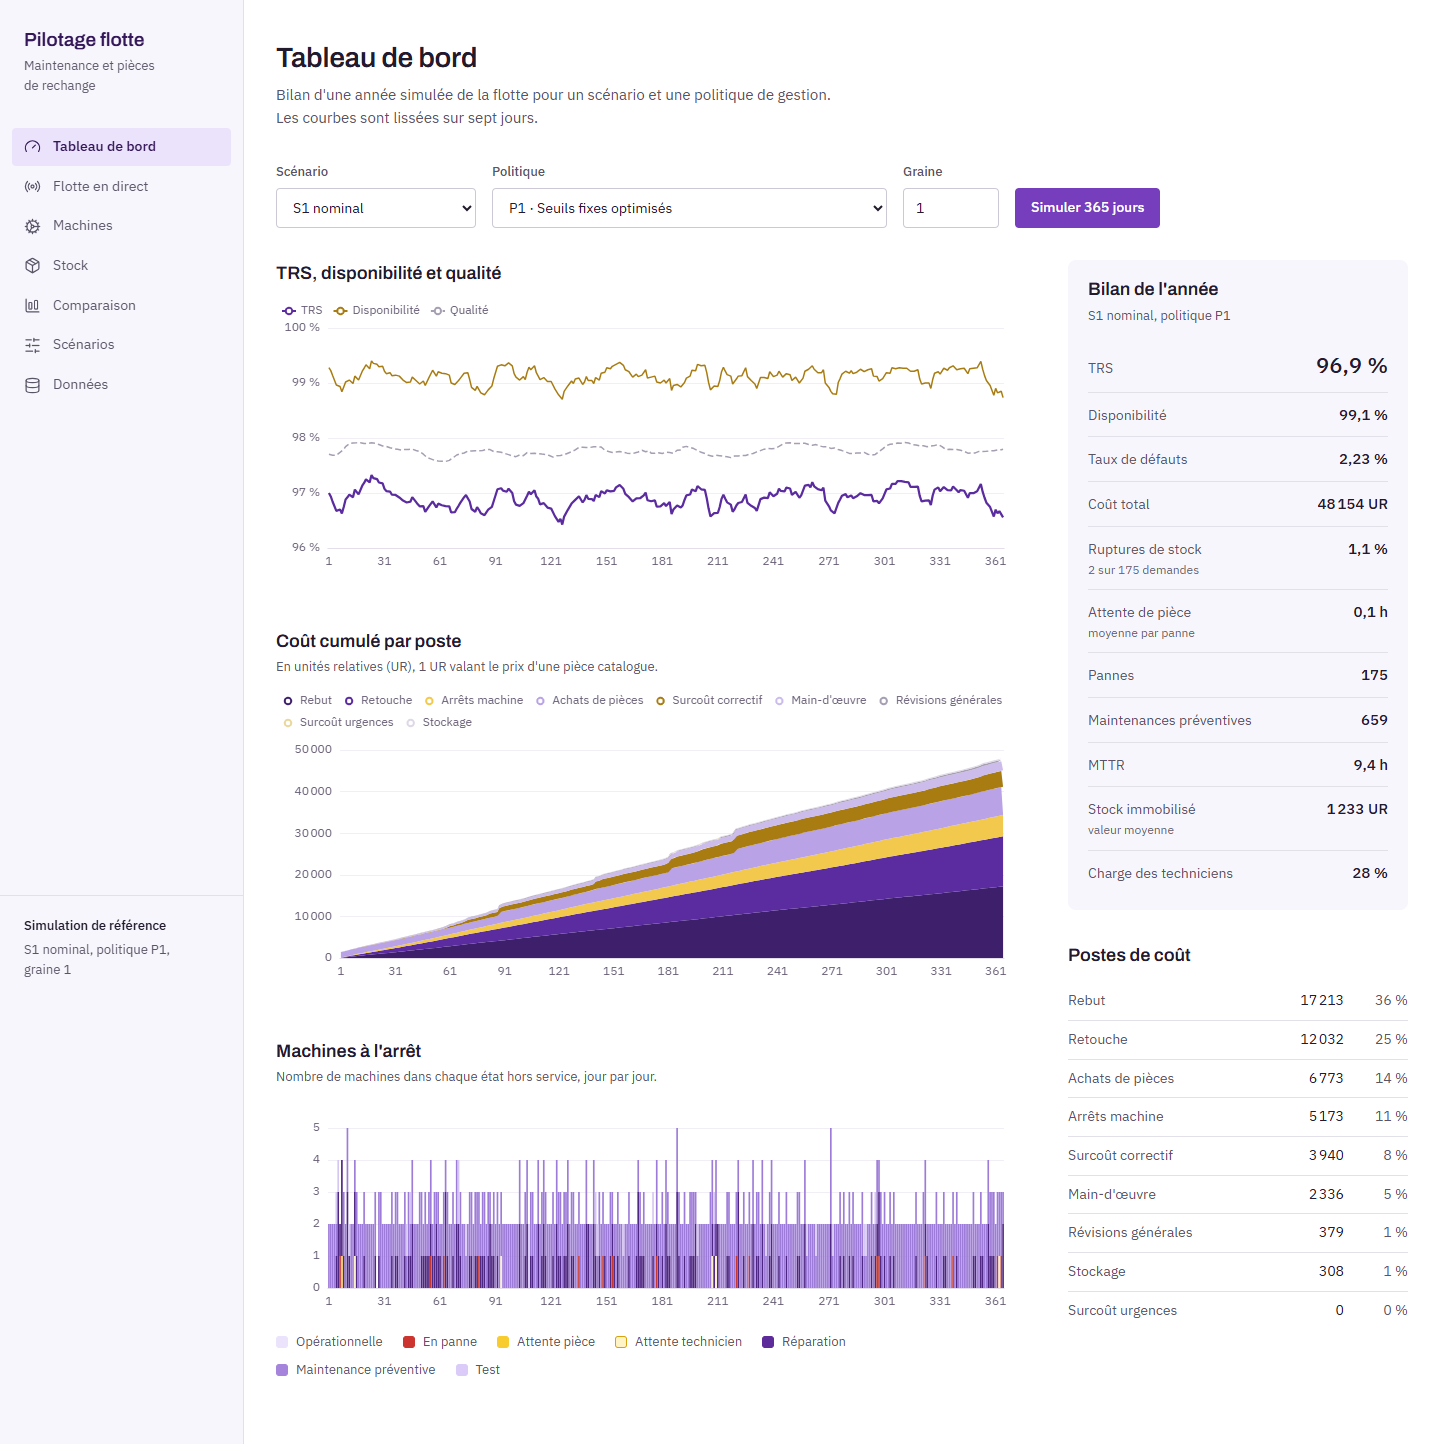
\includegraphics[width=\linewidth]{figures/e2e-dashboard.png}
\caption{Page « Tableau de bord » : bilan d'une année simulée, évolution du TRS, coûts cumulés par poste et machines à l'arrêt.}
\label{fig:web-dashboard}
\end{figure}

\begin{figure}[H]
\centering
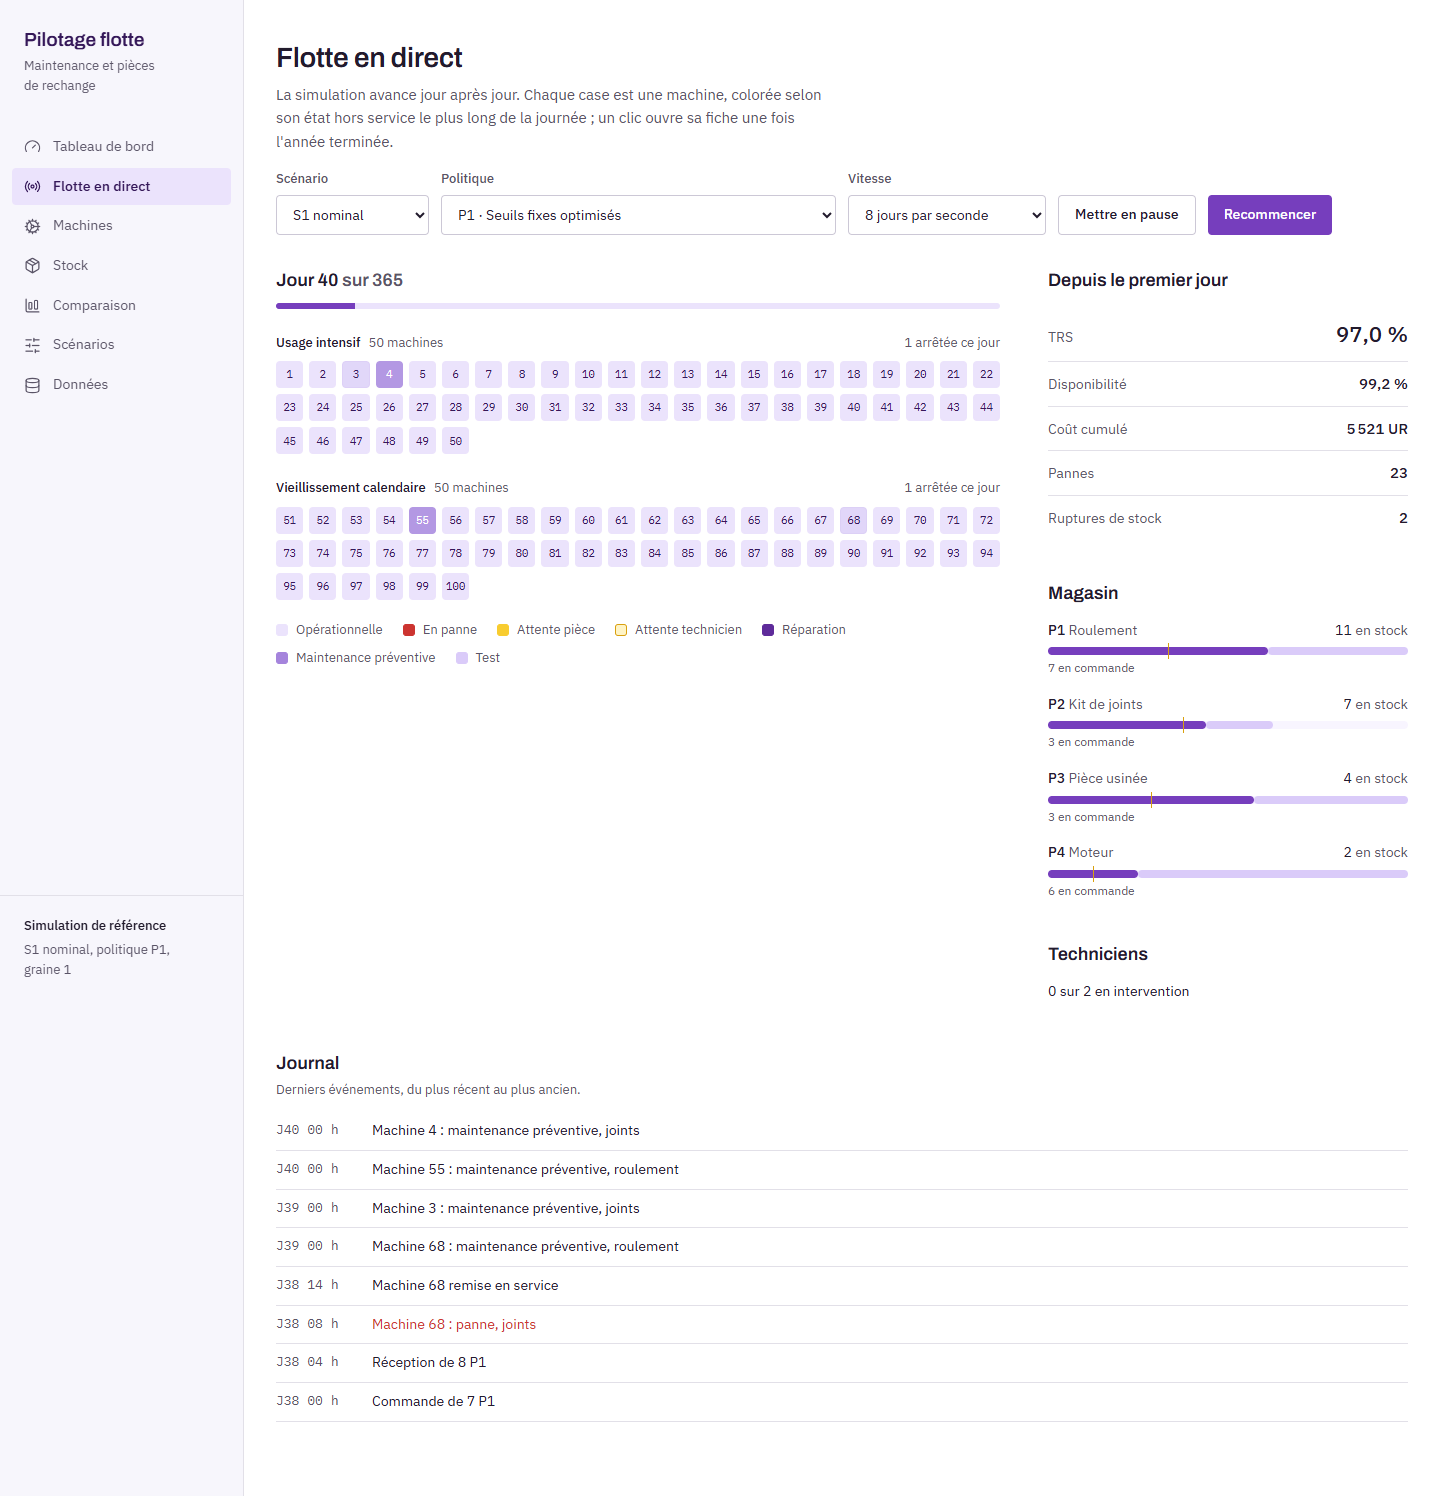
\includegraphics[width=\linewidth]{figures/e2e-live.png}
\caption{Page « Flotte en direct » : la simulation est diffusée jour après jour par WebSocket ; chaque machine est une case colorée selon son état, avec l'état du magasin, la file des techniciens et le journal d'événements rédigé en français.}
\label{fig:web-live}
\end{figure}

\begin{figure}[H]
\centering
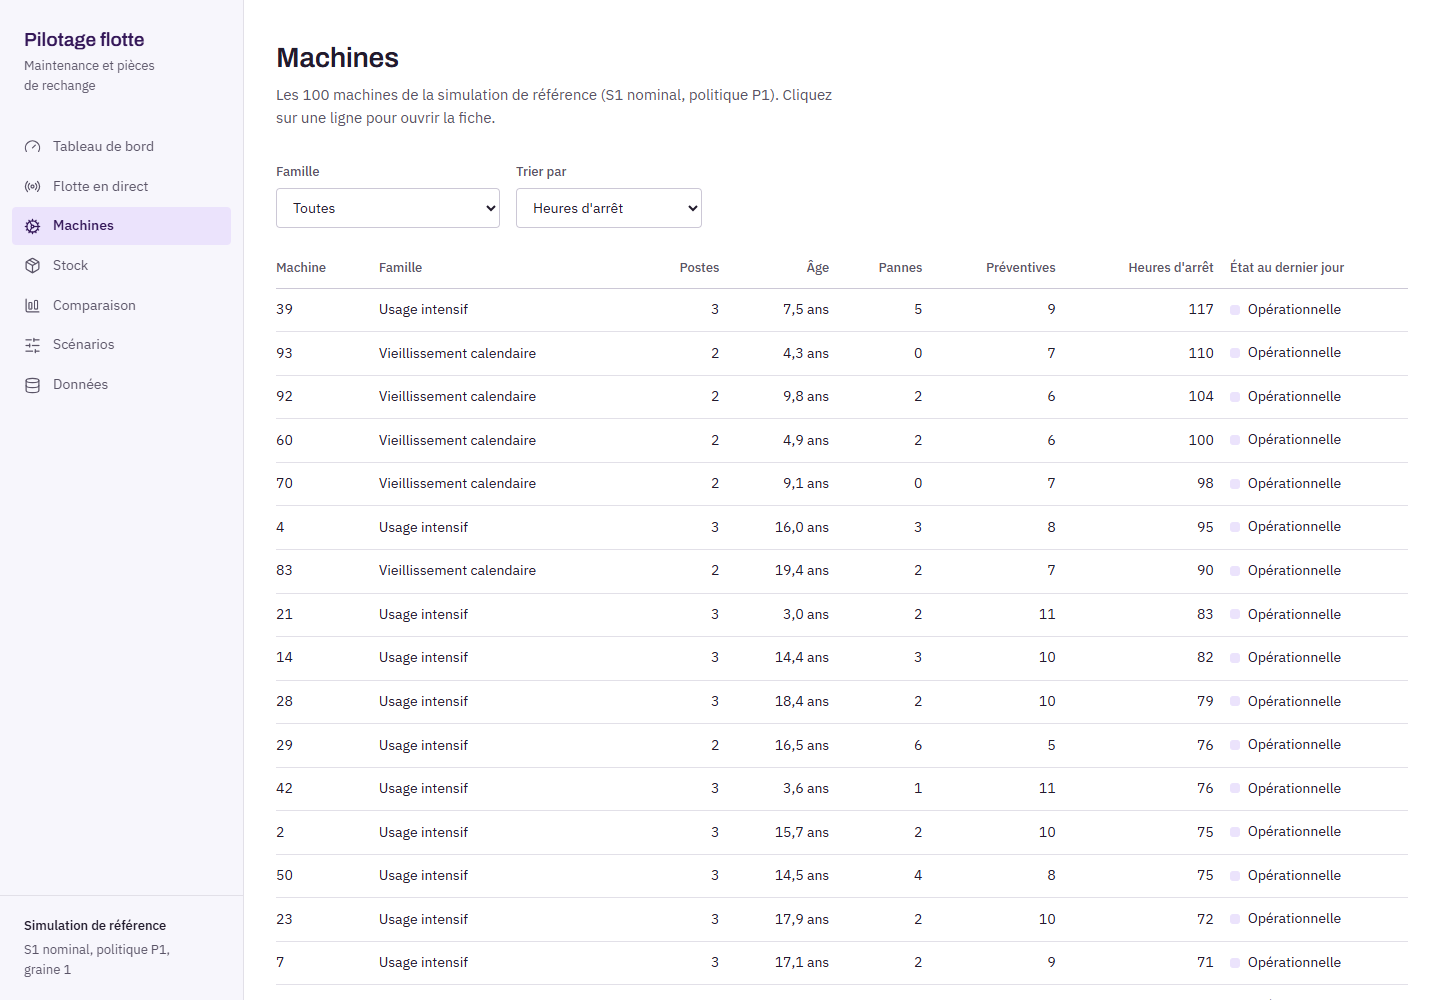
\includegraphics[width=\linewidth]{figures/e2e-machines.png}
\caption{Page « Machines » : les cent machines de la simulation de référence, filtrables par famille et triables par heures d'arrêt, avec pour chacune son âge, son nombre de pannes, ses interventions préventives, ses heures d'arrêt et son état au dernier jour.}
\label{fig:web-machines}
\end{figure}

\begin{figure}[H]
\centering
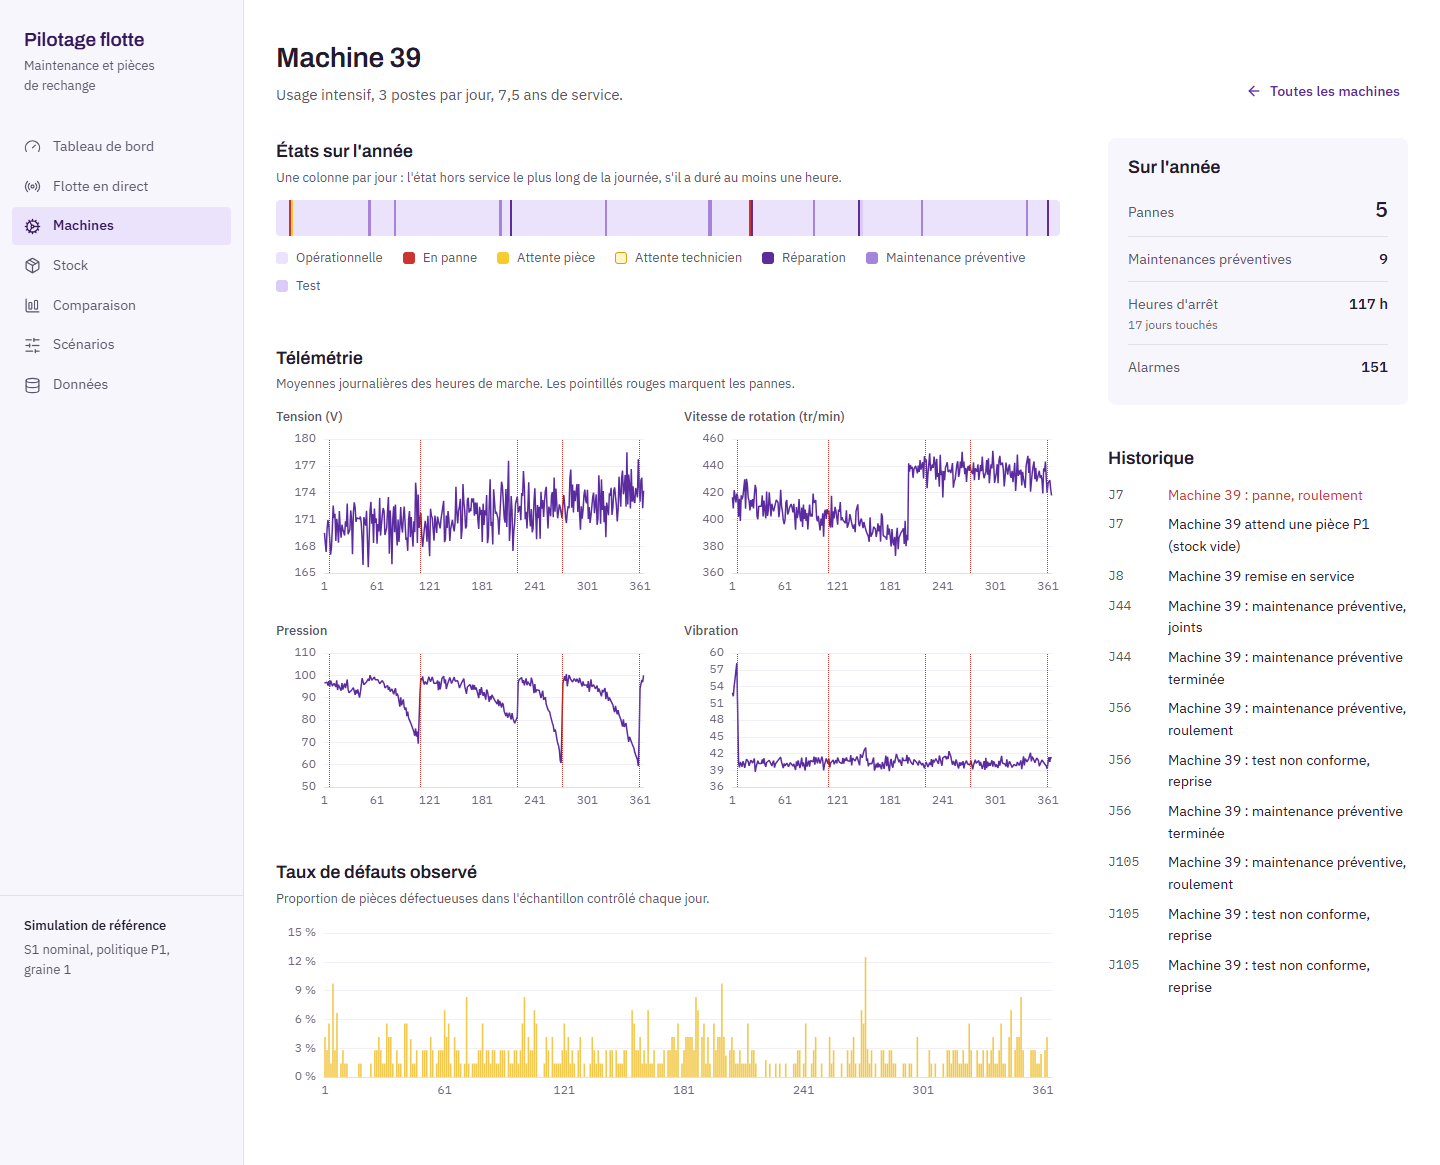
\includegraphics[width=\linewidth]{figures/e2e-machine.png}
\caption{Fiche d'une machine : frise des états sur l'année, télémétrie journalière avec les pannes signalées, taux de défauts observé et historique des interventions.}
\label{fig:web-machine}
\end{figure}

\begin{figure}[H]
\centering
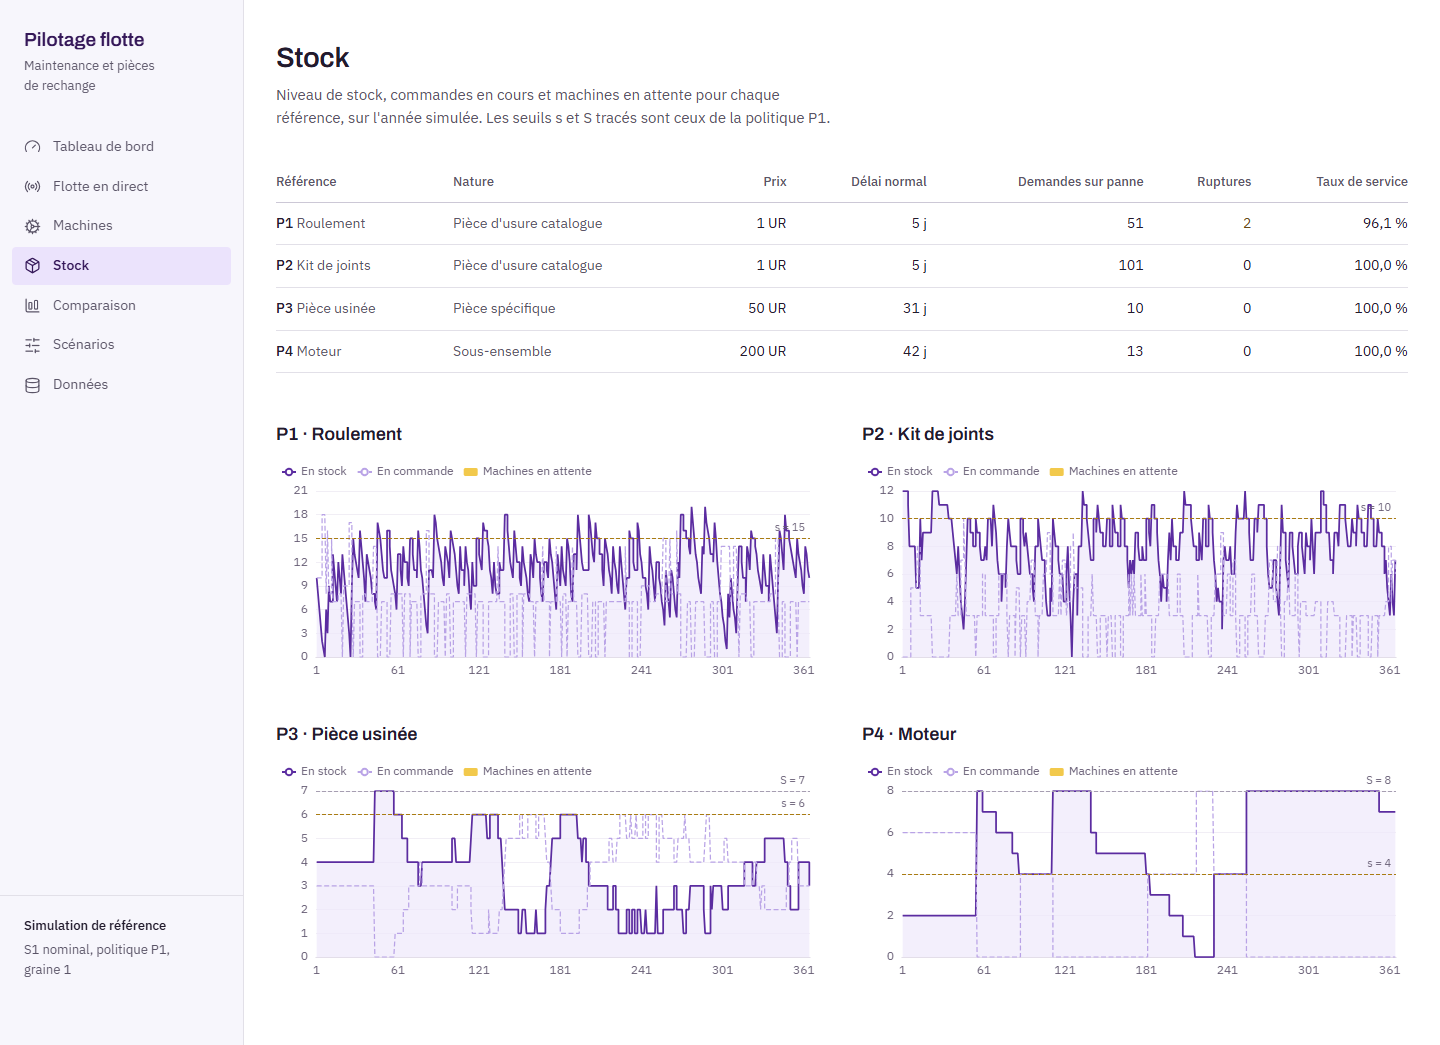
\includegraphics[width=\linewidth]{figures/e2e-stock.png}
\caption{Page « Stock » : niveau, commandes en cours et machines en attente pour chaque référence, avec les seuils de la politique tracés à titre de repère.}
\label{fig:web-stock}
\end{figure}

\begin{figure}[H]
\centering
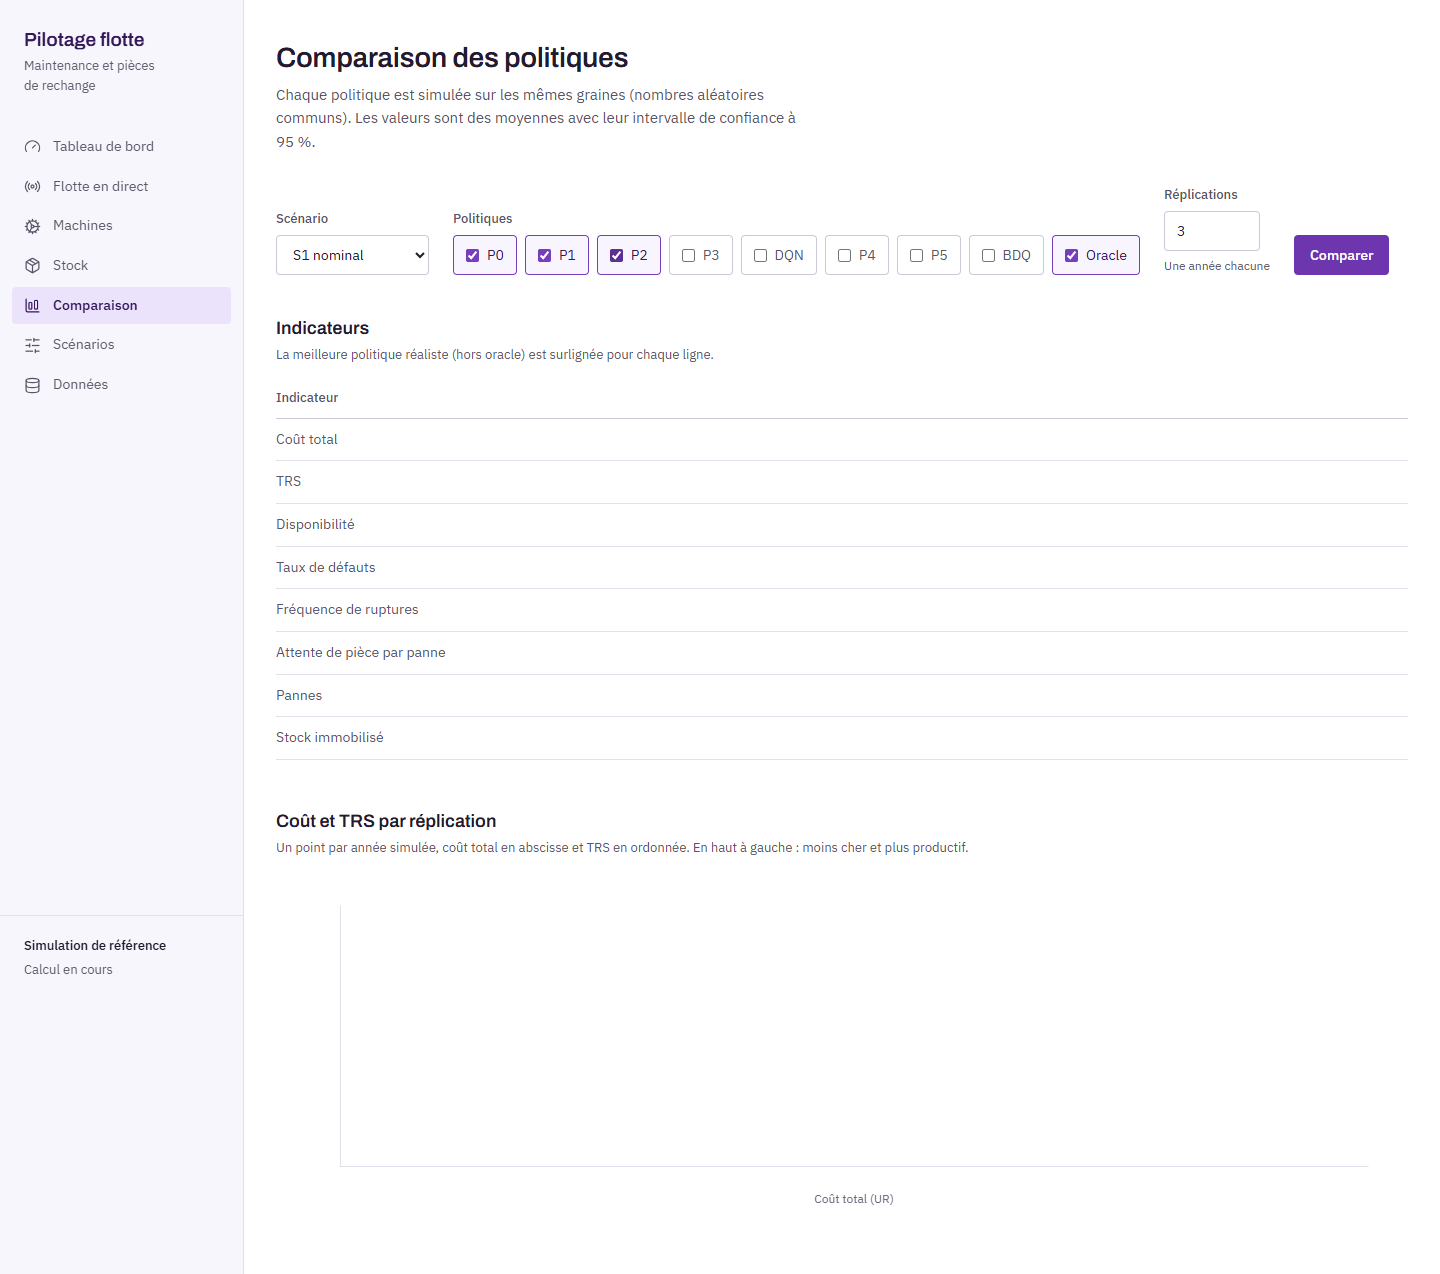
\includegraphics[width=\linewidth]{figures/e2e-compare.png}
\caption{Page « Comparaison » : indicateurs de plusieurs politiques avec intervalles de confiance et nuage coût, TRS réplication par réplication.}
\label{fig:web-compare}
\end{figure}

\begin{figure}[H]
\centering
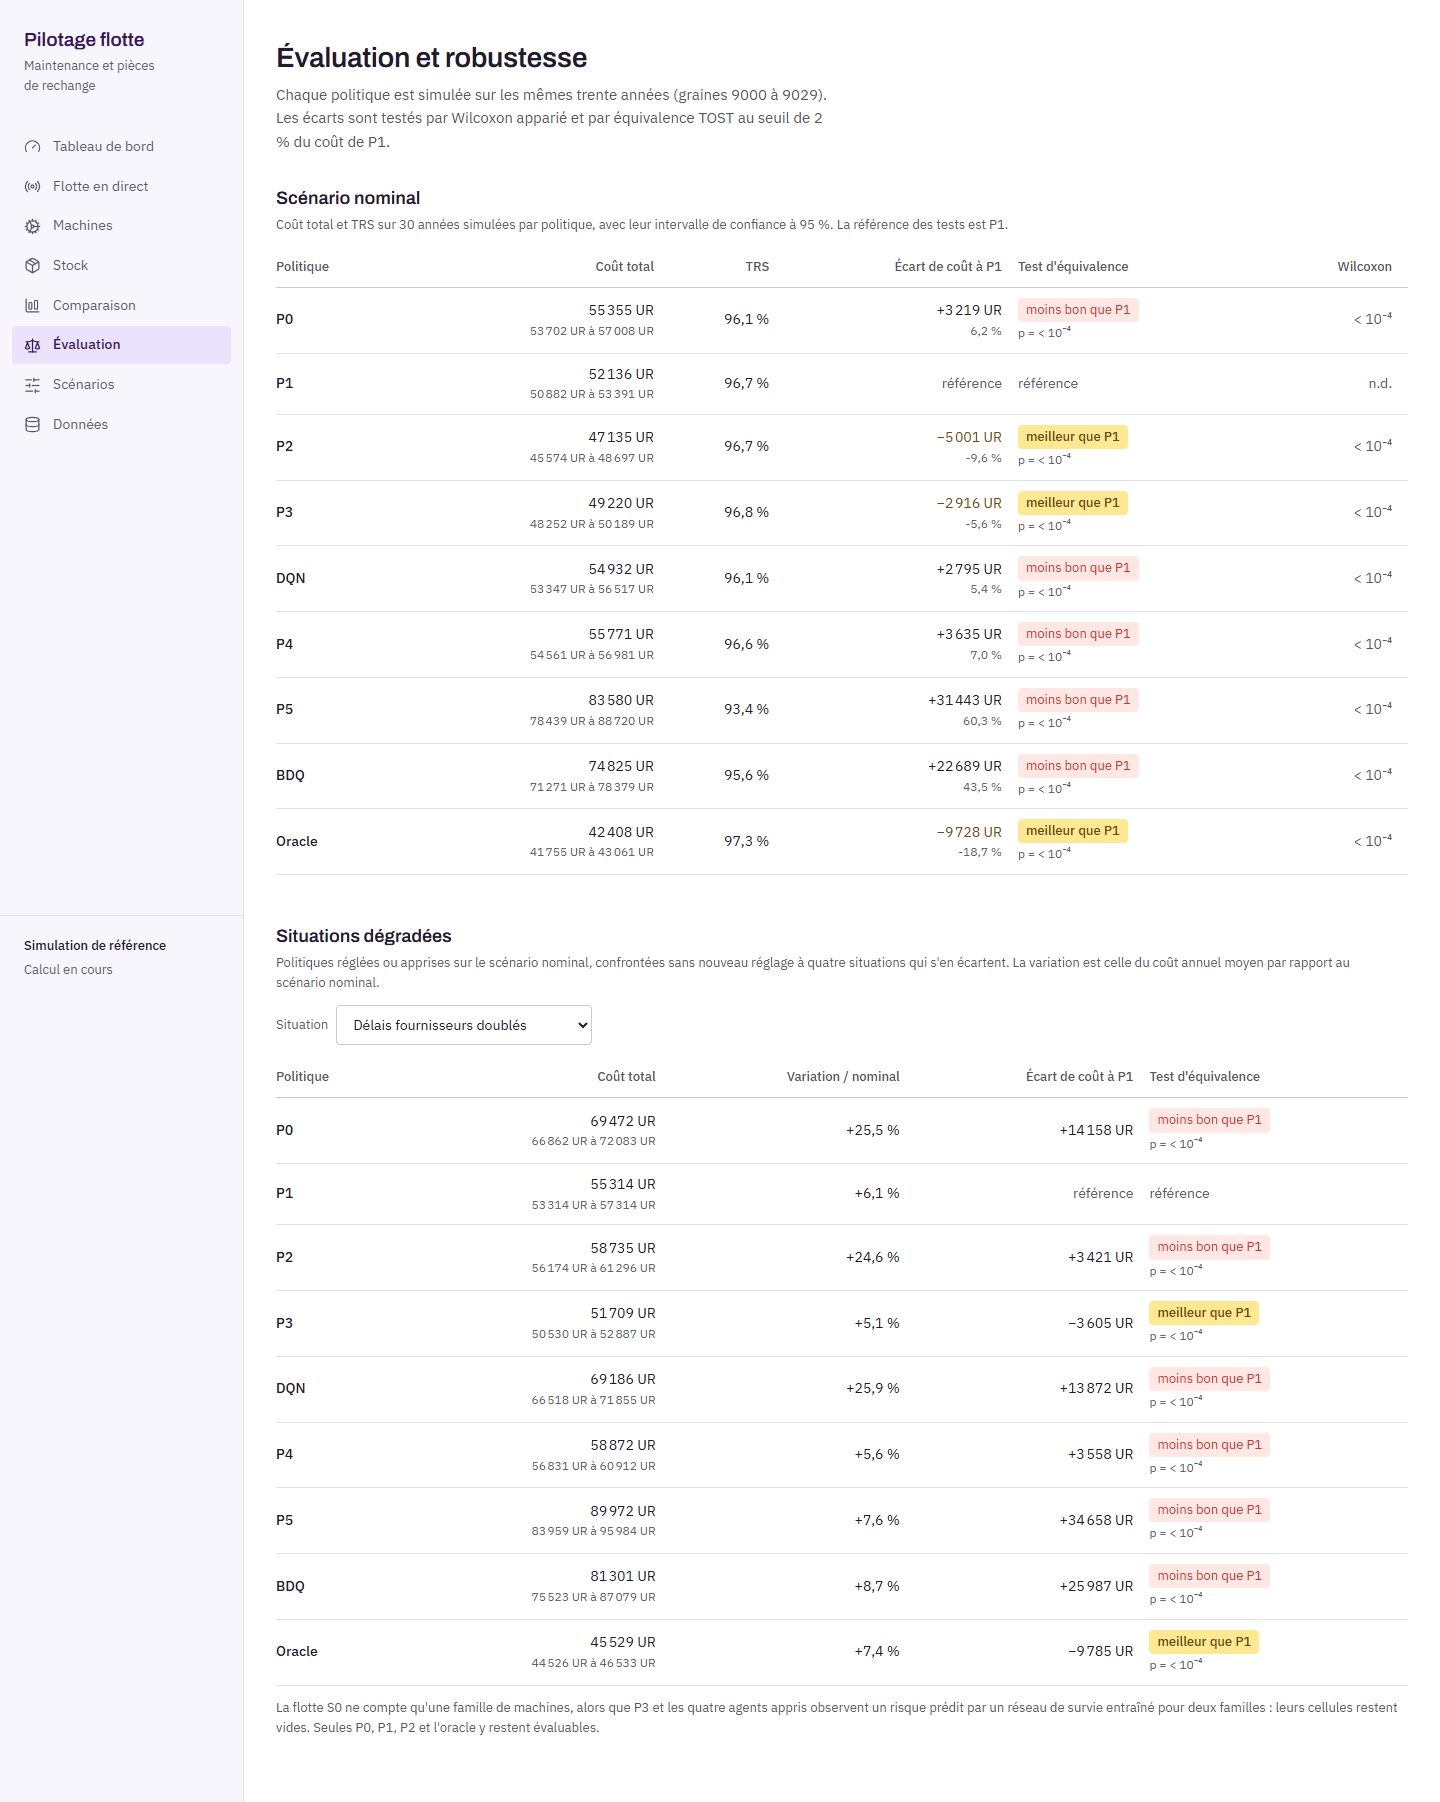
\includegraphics[width=\linewidth]{figures/e2e-evaluation.png}
\caption{Page « Évaluation » : coût, TRS et test d'équivalence au scénario nominal, puis variation du coût et verdict TOST dans la situation dégradée choisie. Les cellules vides signalent les politiques qu'une flotte à famille unique rend inévaluables.}
\label{fig:web-evaluation}
\end{figure}

\begin{figure}[H]
\centering
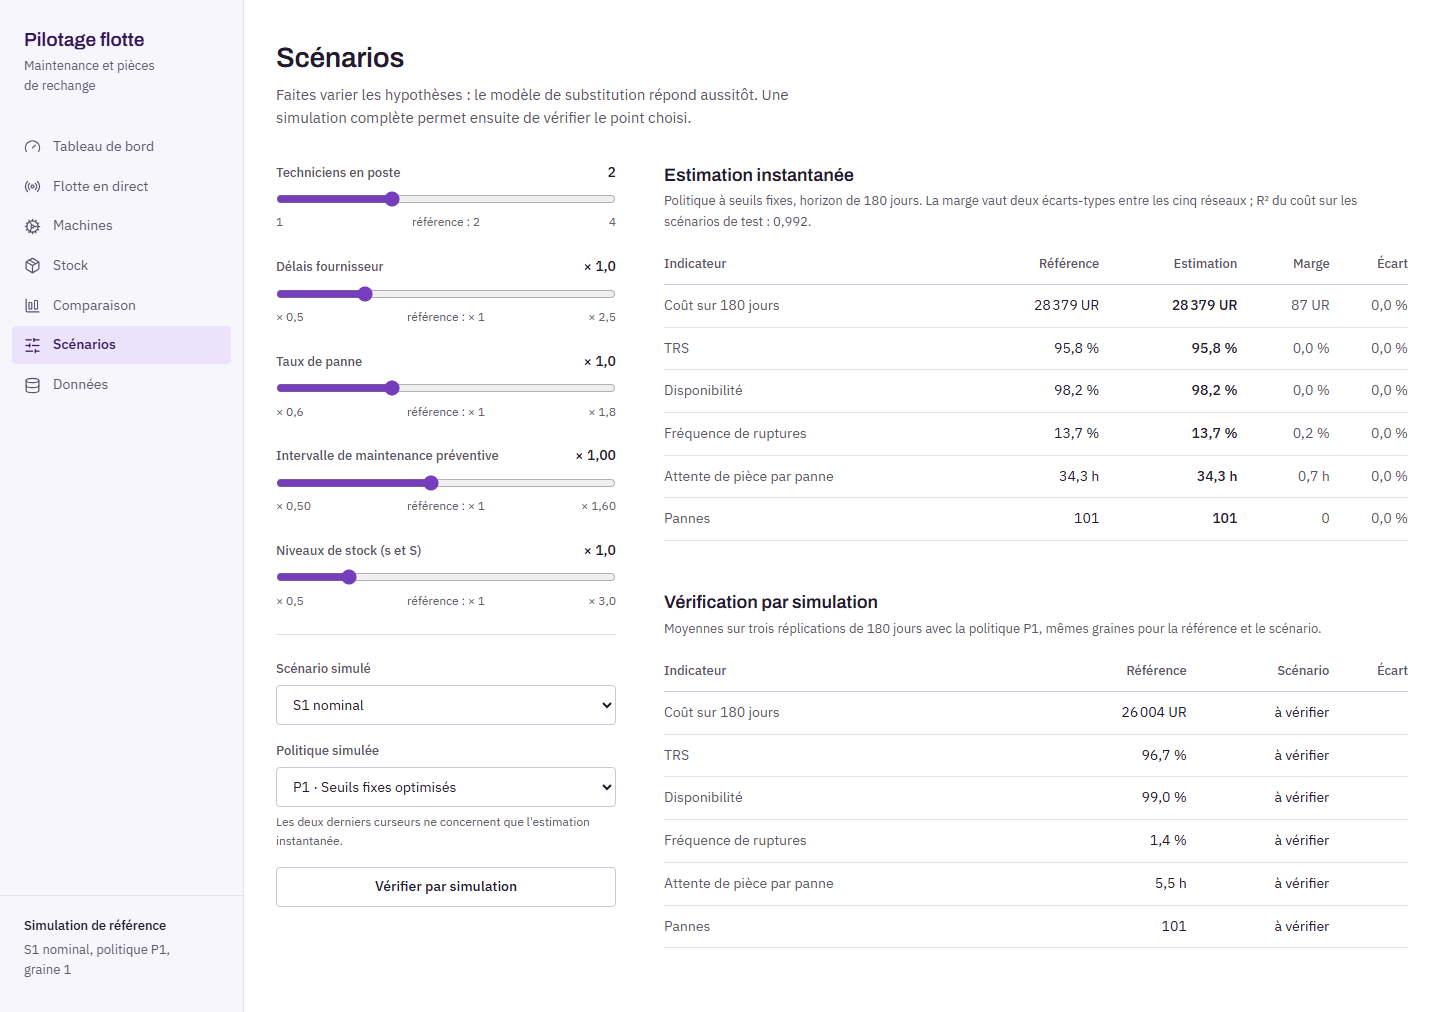
\includegraphics[width=\linewidth]{figures/e2e-scenarios.png}
\caption{Page « Scénarios » : réponse instantanée du modèle de substitution à chaque mouvement de curseur, vérifiable par une simulation complète.}
\label{fig:web-scenarios}
\end{figure}

% ================================================================ Chapitre 6
\chapter{Bilan et perspectives}\label{sec:bilan}

% Bilan, limites et perspectives (sous-sections du chapitre 6)
\subsection{Bilan des objectifs}\label{sec:conclusion}

La question posée par le cahier des charges appelle une réponse nuancée. L'apprentissage profond réduit bien le coût par rapport à une politique à seuils fixes correctement réglée, mais par la prédiction plutôt que par l'apprentissage par renforcement : P3, qui s'appuie sur un réseau de survie, économise 5,6~\% à disponibilité supérieure, et c'est la politique la plus robuste lorsque les délais fournisseurs doublent. Les agents d'apprentissage par renforcement, eux, n'atteignent pas P1 : les deux agents à seuils, P4 et le DQN du niveau réduit, s'en approchent le plus, le premier à 1,3~\% seulement, le second à 5,4~\%. Une règle de maintenance conditionnelle simple fait mieux que toutes les politiques apprises, avec 9,6~\% d'économie.

Deux enseignements en ressortent. Le premier est que la valeur vient de l'information sur l'état des composants : les politiques qui l'exploitent, P2 et P3, divisent le nombre de pannes par quatre à six, et l'oracle montre qu'il reste encore 10~\% à gagner avec une information parfaite. Le second est que l'apprentissage par renforcement bute ici sur des difficultés concrètes, que le projet a rencontrées et levées une à une : un espace d'actions de plus de $10^{76}$ combinaisons, une récompense bruitée par les pannes de toute la flotte, un critique incapable d'apprendre sans normalisation des récompenses, une politique dont l'action la plus probable diffère de la loi apprise. Chacune est documentée avec sa correction, ce qui vaut autant pour la suite que les chiffres eux-mêmes.

\begin{tabularx}{\linewidth}{@{}l L P{3.2cm}@{}}
\caption{Atteinte des objectifs du cahier des charges}\label{tab:objectifs}\\
\toprule
\hd{Obj.} & \hd{Critère et résultat} & \hd{Verdict} \\
\midrule
O1 & Jeu Azure enrichi (durées, familles, défauts, coûts) ; une fuite d'information temporelle détectée, corrigée et couverte par un test & Atteint \\
O2 & Pannes d'Azure reproduites à 10~\% près : écarts de $-$4,3 à $+$7,9~\% sur 2015, jusqu'à 18~\% sur le seul second semestre & Atteint sur l'année \\
O3 & F1 supérieur à LightGBM : vrai aux deux horizons sur données simulées, à 7 jours seulement sur Azure & Atteint en partie \\
O4 & Coût inférieur à P1 à disponibilité au moins égale : meilleur agent (P4) à $+$1,3~\%, DQN à $+$5,4~\% & Non atteint \\
O5 & $R^2$ supérieur à 0,9 sur des scénarios non vus : de 0,964 à 0,994 & Atteint \\
O6 & Application web de neuf pages, parcours principal testé de bout en bout & Atteint \\
\bottomrule
\end{tabularx}

\subsection{Limites}

\begin{itemize}
\item \textbf{Des données réelles elles-mêmes synthétiques.} Le jeu Azure a été généré par Microsoft pour illustrer la maintenance prédictive. Ses pannes sont précédées d'anomalies plus nettes qu'on ne l'observe souvent sur le terrain, ce qui explique en partie le bon score de LightGBM à 24 heures, et sa calibration repose sur une censure informative que nous avons dû corriger par simulation.
\item \textbf{Un simulateur volontairement simplifié.} Les coûts sont exprimés en unités relatives, les fournisseurs n'ont pas de capacité limitée, une pièce déposée n'est jamais réparée ni réutilisée, et les techniciens sont interchangeables.
\item \textbf{Un budget de calcul limité.} Chaque agent est entraîné sur trois graines, chacune en quelques centaines de milliers de pas, sur un poste de travail unique, avec des réglages proches des valeurs usuelles ; parmi elles, la politique retenue est celle dont le coût annuel moyen sur cinq graines de validation est le plus faible, ce qui atténue l'effet d'un tirage particulier sans l'annuler. Un réglage systématique des hyperparamètres et des apprentissages plus longs resteraient nécessaires pour conclure sur les méthodes elles-mêmes.
\item \textbf{Un seul scénario d'apprentissage.} Les agents et les seuils sont réglés sur le scénario nominal ; la robustesse est mesurée sans nouvel apprentissage, ce qui correspond à l'usage réel mais pénalise les politiques les plus spécialisées.
\end{itemize}

\subsection{Perspectives}

\begin{itemize}
\item Donner aux agents du niveau N2 une récompense par machine, qui attribuerait à chaque branche l'effet de sa propre décision : entraîné sur 300\,000 pas, P5 plafonne autour de 67\,000 UR, signe que la durée d'apprentissage n'est plus le facteur limitant.
\item Entraîner les agents sur un ensemble de scénarios tirés au hasard (délais, taux de panne, effectifs) plutôt que sur le seul scénario nominal, pour obtenir des politiques robustes par construction.
\item Remplacer la recherche aléatoire de P1 et la grille de P3 par une optimisation bayésienne sur le modèle de substitution, qui évalue un jeu de paramètres en quelques millisecondes.
\item Confronter le simulateur et les modèles à l'historique d'un atelier réel, qui fournirait les durées, les coûts et les pratiques de maintenance que le jeu Azure ne contient pas.
\end{itemize}


% ================================================================ Conclusion générale
\chapter*{Conclusion générale}
\addcontentsline{toc}{chapter}{Conclusion générale}
\markboth{\textcolor{accent}{Conclusion générale}}{}

Ce travail a parcouru la chaîne complète d'un projet d'ingénierie de la donnée, de la calibration d'un simulateur sur des relevés industriels jusqu'à la restitution d'une décision de maintenance dans une interface web. La réponse à la question du cahier des charges est affirmative, mais elle n'emprunte pas le chemin attendu : c'est la connaissance de l'état des composants, davantage que la méthode d'apprentissage, qui porte l'essentiel du gain. Ce constat, établi sur trente années simulées par politique et vérifié en situation dégradée, invite à investir d'abord dans l'instrumentation et la prédiction, et à n'engager l'apprentissage par renforcement qu'une fois l'espace d'actions et la fonction de récompense maîtrisés.

Au-delà des chiffres, le projet laisse une base réutilisable — simulateur paramétrable, protocole d'évaluation à nombres aléatoires communs, modèle de substitution et banc d'analyse de sensibilité — ainsi qu'un ensemble de difficultés documentées qui, du masquage d'actions à la normalisation des récompenses, intéressent tout pilotage industriel de grande dimension. Le bilan détaillé des objectifs et les perspectives ouvertes par ce travail sont rassemblés au chapitre~\ref{sec:bilan}.

% ================================================================ Bibliographie
\begin{thebibliography}{99}
\addcontentsline{toc}{chapter}{Bibliographie}
\small
\NoAutoSpacing
\setlength{\itemsep}{0.15em}
\bibitem{azure} Microsoft Azure Predictive Maintenance, jeu de données publié sur Kaggle, \url{https://www.kaggle.com/datasets/arnabbiswas1/microsoft-azure-predictive-maintenance}.
\bibitem{gensheimer} M. F. Gensheimer et B. Narasimhan, «~A scalable discrete-time survival model for neural networks~», \emph{PeerJ}, 7:e6257, 2019.
\bibitem{dqn} V. Mnih et al., «~Human-level control through deep reinforcement learning~», \emph{Nature}, 518, p.~529-533, 2015.
\bibitem{ppo} J. Schulman et al., «~Proximal policy optimization algorithms~», arXiv:1707.06347, 2017.
\bibitem{masking} S. Huang et S. Ontañón, «~A closer look at invalid action masking in policy gradient algorithms~», \emph{FLAIRS}, 2022.
\bibitem{bdq} A. Tavakoli, F. Pardo et P. Kormushev, «~Action branching architectures for deep reinforcement learning~», \emph{AAAI}, 2018.
\bibitem{ensembles} B. Lakshminarayanan, A. Pritzel et C. Blundell, «~Simple and scalable predictive uncertainty estimation using deep ensembles~», \emph{NeurIPS}, 2017.
\bibitem{saltelli} A. Saltelli et al., \emph{Global Sensitivity Analysis: The Primer}, Wiley, 2008.
\bibitem{sb3} A. Raffin et al., «~Stable-Baselines3: Reliable reinforcement learning implementations~», \emph{Journal of Machine Learning Research}, 22(268), 2021.
\bibitem{impeccable} Impeccable, catalogue d'anti-modèles d'interface, \url{https://impeccable.style}.
\end{thebibliography}

% ================================================================ Annexes
\appendix

\chapter{Reproduire les résultats}\label{sec:reproduire}

Prérequis : Python 3.11 avec uv, Node.js, une distribution TeX avec XeLaTeX et latexmk (MiKTeX ou TeX Live), les cinq fichiers CSV d'Azure dans \texttt{data/raw}.

\begin{tabularx}{\linewidth}{@{}P{7.2cm} L@{}}
\toprule
\hd{Commande} & \hd{Résultat} \\
\midrule
\texttt{uv sync -{}-extra ml} & Installation des dépendances \\
\texttt{uv run pytest} & Tests automatiques \\
\texttt{uv run uvicorn spareparts.api.app:app} & Serveur de l'API (port 8000) \\
\texttt{npm run dev} (dans \texttt{web}) & Interface de l'application (port 5173) \\
\texttt{npx playwright test} (dans \texttt{web}) & Parcours de bout en bout ; avec \texttt{SHOTS\_DIR}, captures des figures~\ref{fig:web-dashboard} à~\ref{fig:web-scenarios} \\
\texttt{scripts/calibrate\_azure.py} & Lois de Weibull (tableau~\ref{tab:weibull}) \\
\texttt{scripts/validate\_azure.py} & Validation O2 (tableau~\ref{tab:validation}) \\
\texttt{scripts/optimize\_p1.py} & Seuils de P1 \\
\texttt{scripts/train\_predictor.py} & Tableau~\ref{tab:pred-sim} ; avec \texttt{-{}-source azure}, tableau~\ref{tab:pred-azure} \\
\texttt{scripts/tune\_p3.py} & Seuils de P3 \\
\texttt{scripts/train\_rl.py -{}-level n1 -{}-risk -{}-drift -{}-curriculum -{}-seeds 0 1 2} & Agent P4 ; \texttt{-{}-level n2} pour P5 \\
\texttt{scripts/train\_bdq.py -{}-risk -{}-drift} \newline \texttt{-{}-curriculum -{}-seeds 0 1 2} & Branching Dueling Q-Network \\
\texttt{scripts/train\_rl.py -{}-level reduced -{}-algo dqn} \newline \texttt{-{}-risk -{}-drift -{}-curriculum -{}-seeds 0 1 2} & DQN du niveau réduit \\
\texttt{scripts/choose\_agent\_mode.py} & Mode de jeu de P4 et P5 \\
\texttt{scripts/train\_surrogate.py} & Modèle de substitution \\
\texttt{scripts/sensitivity.py} & Indices de Sobol (figure~\ref{fig:sobol}, tableau~\ref{tab:sobol}) \\
\texttt{scripts/evaluate\_policies.py -{}-robustness} & Évaluation finale (chapitre~\ref{sec:evaluation}) \\
\texttt{scripts/generate\_fleets.py -{}-n 5} & Compositions de flotte (tableau~\ref{tab:generalisation}) \\
\texttt{scripts/generalize\_ranking.py} & Généralisation du classement (tableau~\ref{tab:generalisation}, figure~\ref{fig:generalisation}) \\
\texttt{scripts/export\_report\_data.py} & Données des graphiques de ce rapport \\
\texttt{latexmk -xelatex rapport.tex} (dans \texttt{docs/rapport}) & Ce rapport en PDF ; latexmk relance XeLaTeX jusqu'à ce que sommaire, listes et références soient stables \\
\bottomrule
\end{tabularx}

\section{Graines aléatoires}\label{sec:graines}

Chaque étape du projet dispose de sa plage de graines, et les plages restent disjointes pour qu'une politique ne soit jamais évaluée sur les années qui ont servi à la régler. La calibration des lois de durée de vie emploie les graines 0 à 3, le jeu d'apprentissage de la prédiction les graines 1 à 5 (cinq années simulées), le réglage de P1, de P3 et du mode de jeu des agents les graines 101 à 103, la sélection du meilleur modèle des agents appris les graines 8\,000 à 8\,004, et l'évaluation finale, comme la robustesse, les graines 9\,000 à 9\,029. Chaque agent est en outre entraîné sur trois graines indépendantes (0, 1 et 2) ; la dispersion qui en résulte est étudiée à la figure~\ref{fig:dispersion}.

À l'intérieur d'une campagne, la même graine produit les mêmes pannes pour toutes les politiques : les politiques affrontent donc les mêmes années, et l'écart de coût qui les sépare tient à la politique et non au tirage. C'est ce qui autorise les tests appariés du chapitre~\ref{sec:evaluation}, et c'est aussi pourquoi les graines d'évaluation sont prises au-delà de toutes celles du réglage et de la sélection.

\section{Journal des campagnes}\label{sec:journal}

Ce journal fixe la chronologie des campagnes qui ont produit les résultats du rapport et les
décisions prises à chaque étape. Il complète les commandes de la section précédente et les graines
de la section~\ref{sec:graines} : ces trois rubriques suffisent à reconstituer l'état du dépôt.
Chaque ligne rapporte une campagne réellement exécutée, avec la valeur mesurée — y compris
lorsqu'elle est défavorable, comme l'optimisation sur modèle de substitution.

\begin{tabularx}{\linewidth}{@{}P{1.9cm} P{4.0cm} L@{}}
\caption{Journal des campagnes, de l'outillage à l'état final du dépôt}\label{tab:journal}\\
\toprule
\hd{Date} & \hd{Campagne} & \hd{Décision et état du dépôt} \\
\midrule
3~nov.~2026 & Outillage de restitution & Tableau d'équivalence \ref{tab:tost}, indices de Sobol \ref{tab:sobol} et gardien de cohérence rapport~$\leftrightarrow$~données : les conventions de restitution (marge $\pm 2$~\%, annualisation des courbes) sont figées par des tests. \\
\addlinespace
3~nov.~2026 & Options d'apprentissage & Récompense par branche au niveau N2, masquage guidé par le risque et entraînement multi-scénarios. Activation explicite ; le défaut reste inchangé pour que les modèles publiés demeurent reproductibles. \\
\addlinespace
3~nov.~2026 & Optimisation bayésienne & Le modèle de substitution place l'optimum à 26\,818~UR, que le simulateur porte à 56\,457~UR : résultat négatif, il ne bat pas la recherche aléatoire (53\,684~UR). La recherche aléatoire est conservée pour P1. \\
\addlinespace
3~nov.~2026 & Généralisation & Cinq compositions de flotte rejouées : P1 et P3 réglés composition par composition, les autres politiques transférées. L'ordre attendu est conservé sur quatre compositions sur six (tableau~\ref{tab:generalisation}). \\
\addlinespace
4~nov.~2026 & Réentraînement et artefacts & P4 (MaskablePPO N1) et P5 (MaskablePPO N2) réentraînés, puis régénération de tous les artefacts (évaluation, robustesse, Sobol, plancher, généralisation, courbes) à partir des modèles retenus. \\
\addlinespace
4~nov.~2026 & Couverture des tests & Campagne de tests : la suite passe de 82 à 128 tests, aucun ignoré, et la couverture de 85,50~\% à 94,19~\%, au-dessus du seuil de 80~\%. \\
\addlinespace
4~nov.~2026 & Compilation du rapport & Le binaire XeLaTeX plante dans l'environnement d'automatisation ; la compilation du PDF est déléguée au job « Rapport (XeLaTeX) » de la chaîne d'intégration. \\
\addlinespace
8~nov.~2026 & Revue de robustesse & Normalisation Azure restreinte à la seule période d'apprentissage, WebSocket borné par un délai d'attente et fermé proprement, CORS limité aux origines locales, taille d'effet $d_z$ déclarée non estimable au lieu de nulle, invariant de révision rendu explicite sous \texttt{python -O}. La suite compte désormais 136 tests, aucun ignoré, pour une couverture de 93,91~\%. \\
\bottomrule
\end{tabularx}

L'état final est celui du 8~novembre~2026 : les agents publiés sont les modèles retenus à l'issue
des campagnes d'apprentissage, les artefacts du rapport sont régénérés à partir de ces modèles, la
suite de tests est verte et le PDF est compilé sans erreur.
Le détail des commandes figure dans la section précédente, celui des
plages de graines dans la section~\ref{sec:graines}.

\chapter{Dictionnaire des données}\label{sec:dictionnaire-annexe}

Le tableau~\ref{tab:dictionnaire} décrit les principales colonnes du jeu de données enrichi (livrable O1). La colonne « Origine » distingue les valeurs issues du jeu Azure, celles estimées par calibration (lois de Weibull, familles) et celles produites par le simulateur.

\begin{tabularx}{\linewidth}{@{}P{3.0cm} P{2.3cm} P{1.5cm} L@{}}
\caption{Colonnes du jeu de données enrichi}\label{tab:dictionnaire}\\
\toprule
\hd{Colonne} & \hd{Type} & \hd{Unité} & \hd{Origine et description} \\
\midrule
\multicolumn{4}{@{}l}{\hd{machines}}\\
machine\_id & entier & --- & Azure : identifiant de la machine (1 à 100) \\
model & entier & --- & Azure : modèle (3, 4, 25 ou 35) \\
age\_years & réel & an & Azure : âge de la machine (0 à 20) \\
family & catégorie & --- & Calibration : famille U (usure) ou C (calendaire) \\
shifts & entier & --- & Hypothèse : nombre de postes de 8 h par jour \\
cadence & entier & pièces/h & Hypothèse : cadence en heures de marche \\
defect\_base & réel & --- & Hypothèse : taux de défaut de base $p_0$ \\
\midrule
\multicolumn{4}{@{}l}{\hd{components}}\\
component & catégorie & --- & Calibration : comp1 à comp4 \\
regime & catégorie & --- & Hypothèse : usure (R1) ou calendaire (R2) \\
pm\_interval & réel & h & Hypothèse : intervalle de maintenance préventive \\
weibull\_beta, weibull\_eta & réel & ---, h & Calibration : forme et échelle (tableau~\ref{tab:weibull}) \\
signal & catégorie & --- & Hypothèse : signal précurseur (tension, rotation, pression, vibration) \\
\midrule
\multicolumn{4}{@{}l}{\hd{parts}}\\
part\_id & entier & --- & Hypothèse : référence de pièce \\
price & réel & UR & Hypothèse : prix unitaire \\
lead\_mu, lead\_cv & réel & h, --- & Hypothèse : délai fournisseur (log-normale) \\
s, S & entier & pièces & Hypothèse ou politique : seuils de recomplètement \\
\midrule
\multicolumn{4}{@{}l}{\hd{technicians}}\\
technicians & entier & --- & Hypothèse : effectif (2 dans le scénario nominal) \\
cost\_hour & réel & UR/h & Hypothèse : coût horaire d'un technicien \\
\midrule
\multicolumn{4}{@{}l}{\hd{production}}\\
machine\_id, hour & entier & --- & Simulateur : machine et heure de production \\
produced & entier & pièces & Simulateur : pièces produites \\
defective & entier & pièces & Simulateur : pièces défectueuses \\
scrapped, reworked & entier & pièces & Simulateur : rebutées et retouchées \\
\midrule
\multicolumn{4}{@{}l}{\hd{quality\_events}}\\
event\_id & entier & --- & Simulateur : identifiant du défaut détecté \\
defect\_type & catégorie & --- & Simulateur : mode de défaut \\
suspected\_\allowbreak component & catégorie & --- & Simulateur : composant suspecté \\
decision & catégorie & --- & Simulateur : rebut ou retouche \\
\midrule
\multicolumn{4}{@{}l}{\hd{events}}\\
timestamp & horodatage & --- & Simulateur : instant de l'événement (h) \\
machine\_id & entier & --- & Simulateur : machine concernée \\
event\_type & catégorie & --- & Simulateur : panne, correctif, préventif, commande, livraison \\
duration, cost & réel & h, UR & Simulateur : durée et coût de l'événement \\
\midrule
\multicolumn{4}{@{}l}{\hd{state\_intervals}}\\
machine\_id & entier & --- & Simulateur : machine concernée \\
state & catégorie & --- & Simulateur : état (en marche, panne, attente pièce, attente technicien, maintenance, arrêt) \\
start, end & réel & h & Simulateur : début et fin du séjour, continus par machine \\
cause & catégorie & --- & Simulateur : cause de l'entrée dans l'état \\
\midrule
\multicolumn{4}{@{}l}{\hd{ml\_features}}\\
signal\_mean\_3h, signal\_std\_24h & réel & --- & Azure et simulateur : statistiques glissantes \\
errors\_24h, defect\_rate\_8h & entier, réel & ---, \% & Azure et simulateur : erreurs et taux de défauts \\
hours\_since\_pm & réel & h & Simulateur : temps écoulé depuis le dernier remplacement \\
turns\_since\_pm & réel & $10^6$ tours & Simulateur : rotation cumulée en heures de marche \\
time\_to\_pm & réel & h & Simulateur : distance à l'échéance de maintenance \\
usage\_rate & réel & --- & Simulateur : taux d'utilisation de la machine \\
stock, on\_order, eta & entier, horodatage & pièces, --- & Simulateur : contexte logistique \\
fail\_24h, fail\_7d, time\_to\_failure, censored & entier, réel, booléen & ---, h, --- & Étiquettes de survie et indicateur de censure \\
\bottomrule
\end{tabularx}

\end{document}
